% Wolf Prize in Mathematics — ALL IN ONE（合集）
% 汇集 episode-02 ~ episode-12 为单一文档：沃尔夫数学奖人物谱系
% 复用各集的 personslide / portraitbox 宏（以 Style-B 为准，Style-A 用 personslideA 兼容）
% Source: Wolf_Prize/video/episode-02..12 离线页面
\documentclass[aspectratio=169,14pt]{beamer}
\usetheme{default}\usecolortheme{default}\setbeamertemplate{navigation symbols}{}
\setbeamertemplate{footline}{\hfill{\scriptsize\color{covermuted}\insertframenumber/\inserttotalframenumber}\hspace{0.4cm}\vspace{0.15cm}}
\usepackage{fontspec}\usepackage{xeCJK}\setCJKmainfont{PingFang SC}[BoldFont=PingFang SC Semibold]\setmainfont{Helvetica Neue}[BoldFont=Helvetica Neue Bold]
\usepackage{xcolor}\usepackage{tikz}\usepackage{graphicx}\usepackage{fontawesome5}\usepackage{amssymb}\usetikzlibrary{positioning,calc,arrows.meta,shadows}\def\crosscontent{}
\definecolor{bgmain}{RGB}{238,243,252}\definecolor{panel}{RGB}{238,244,255}\definecolor{factbg}{RGB}{246,242,235}\definecolor{coverprimary}{HTML}{2563EB}\definecolor{coveraccent}{HTML}{00A884}\definecolor{coverwarning}{HTML}{F59E0B}\definecolor{coverdark}{HTML}{1F2937}\definecolor{covermuted}{HTML}{64748B}\definecolor{titlecolor}{RGB}{30,30,30}\definecolor{muteddark}{RGB}{72,86,115}\definecolor{bluepanel}{RGB}{226,237,255}\definecolor{greenpanel}{RGB}{225,246,237}\definecolor{amberpanel}{RGB}{255,244,222}\definecolor{purplepanel}{RGB}{239,231,255}\setbeamercolor{background canvas}{bg=bgmain}
\definecolor{coverlight}{RGB}{229,237,234}
% ---- 交叉殊荣页：颜色定义（与 turing/copss 卡片矩阵一致）----
\definecolor{wolfclr}{RGB}{180,120,0}      % 沃尔夫金
\definecolor{wolfbg}{RGB}{232,240,250}      % 浅蓝底
\definecolor{fieldsclr}{RGB}{41,65,122}
\definecolor{abelclr}{RGB}{150,40,90}
\definecolor{chernclr}{RGB}{15,110,92}
\definecolor{turingclr}{RGB}{41,65,122}
\definecolor{copssclr}{RGB}{33,102,172}
\definecolor{mutedgray}{RGB}{100,100,100}
% 交叉殊荣页：居中标题模板（与 turing/copss 一致）
\newcommand{\framesubject}{}
\setbeamertemplate{frametitle}{%
  \vspace{8pt}%
  \centering
  {\fontsize{13}{15}\selectfont\bfseries\color{coverprimary}沃尔夫数学奖 · \insertframetitle}\\[3pt]
  \textcolor{wolfbg}{\rule{0.95\textwidth}{0.6pt}}%
  \vspace{-6pt}%
}
\newcommand{\plainbar}{\begin{tikzpicture}[remember picture, overlay]\fill[coverdark, opacity=0.07] (current page.south west) rectangle ([yshift=0.4cm]current page.south east);\draw[coveraccent, opacity=0.45, line width=0.8pt] ([yshift=0.4cm]current page.south west) -- ([yshift=0.4cm]current page.south east);\end{tikzpicture}}
\newcommand{\deckbackground}{\begin{tikzpicture}[remember picture, overlay]\fill[coverprimary!8] (current page.north west) rectangle (current page.south east);\fill[coverprimary!14] (current page.north west) ++(1.55,-1.35) circle (2.45cm);\fill[coveraccent!12] (current page.south east) ++(-1.9,1.45) circle (2.70cm);\fill[coverwarning!12] (current page.north east) ++(-2.9,-1.8) circle (0.85cm);\foreach \x in {-0.2,0.8,...,16.2} {\draw[coverprimary, opacity=0.045, line width=0.25pt] ([xshift=\x cm]current page.south west) -- ([xshift=\x cm]current page.north west);}\foreach \y in {-0.2,0.7,...,9.3} {\draw[coverprimary, opacity=0.04, line width=0.25pt] ([yshift=\y cm]current page.south west) -- ([yshift=\y cm]current page.south east);}\draw[coveraccent, opacity=0.38, line width=1.1pt] ([xshift=0.35cm,yshift=7.72cm]current page.south west) -- ++(3.25,0) -- ++(0.45,-0.45) -- ++(2.0,0);\draw[coverprimary, opacity=0.24, line width=1.0pt] ([xshift=9.35cm,yshift=8.25cm]current page.south west) -- ++(2.3,0) -- ++(0.55,-0.55) -- ++(3.2,0);\fill[coverdark, opacity=0.07] (current page.south west) rectangle ([yshift=0.42cm]current page.south east);\end{tikzpicture}}
\newcommand{\sectiontitle}[2]{\vspace{-0.52cm}\begin{center}{\fontsize{20}{24}\selectfont\bfseries\color{titlecolor} #1}\\[2pt]{\fontsize{9}{11}\selectfont\itshape\color{muteddark} #2}\end{center}\vspace{0.12cm}}
\newcommand{\portraitbox}[2]{\begin{tikzpicture}\node[draw=coverprimary!28, line width=0.7pt, fill=white, rounded corners=3pt, inner sep=2.5pt, drop shadow={shadow xshift=0.5pt, shadow yshift=-0.5pt, opacity=0.12}] {\includegraphics[width=2.4cm,height=2.9cm,keepaspectratio]{#1}};\end{tikzpicture}{\par\vspace{1pt}\fontsize{6.5}{7.5}\selectfont\color{covermuted} #2\par}}
\newcommand{\placeholderportrait}[2]{\begin{tikzpicture}\node[draw=coverprimary!28, line width=0.7pt, fill=white, rounded corners=3pt, inner sep=2.5pt, drop shadow={shadow xshift=0.5pt, shadow yshift=-0.5pt, opacity=0.12}] {\begin{tikzpicture}\fill[bluepanel] (0,0) rectangle (2.4,2.9);\foreach \x/\y in {0.25/0.45,0.55/1.85,0.95/1.15,1.35/2.2,1.75/0.85,2.1/1.65} {\fill[coverprimary!32] (\x,\y) circle (0.055cm);}\draw[coveraccent!45, line width=0.55pt] (0.25,0.45) -- (0.55,1.85) -- (0.95,1.15) -- (1.35,2.2) -- (1.75,0.85) -- (2.1,1.65);\node[circle, fill=coverprimary!16, minimum size=0.78cm] at (1.2,1.78) {};\node[rounded corners=8pt, fill=coverprimary!16, minimum width=1.28cm, minimum height=0.72cm] at (1.2,0.78) {};\node[font=\fontsize{12}{14}\selectfont\bfseries, text=coverprimary!75!black] at (1.2,0.17) {#1};\end{tikzpicture}};\end{tikzpicture}{\par\vspace{1pt}\fontsize{6.5}{7.5}\selectfont\color{covermuted} #2\par}}
\newcommand{\personslide}[9]{\begin{frame}\plainbar\vspace{-0.45cm}\begin{center}{\fontsize{22}{26}\selectfont\bfseries\color{coverdark} #1}\\[2pt]{\fontsize{9.5}{11.5}\selectfont\color{muteddark} #2}\end{center}\vspace{0.15cm}\begin{columns}[c]\begin{column}{0.22\textwidth}\centering #3\end{column}\begin{column}{0.28\textwidth}\begin{tikzpicture}\node[fill=greenpanel, rounded corners=4pt, inner xsep=6pt, inner ysep=5pt, text width=3.8cm, align=left] {{\fontsize{7}{8.5}\selectfont\bfseries\color{coveraccent!70!black} 获奖}\enspace{\fontsize{7}{8.5}\selectfont\color{coverdark!85} #4}\\[2.5pt]{\fontsize{7}{8.5}\selectfont\bfseries\color{coveraccent!70!black} 生卒}\enspace{\fontsize{7}{8.5}\selectfont\color{coverdark!85} #5}\\[2.5pt]{\fontsize{7}{8.5}\selectfont\bfseries\color{coveraccent!70!black} 身份}\enspace{\fontsize{7}{8.5}\selectfont\color{coverdark!85} #6}\\[2.5pt]{\fontsize{7}{8.5}\selectfont\bfseries\color{coveraccent!70!black} 机构}\enspace{\fontsize{7}{8.5}\selectfont\color{coverdark!85} #7}};\end{tikzpicture}\crosscontent\end{column}\begin{column}{0.48\textwidth}\begin{tikzpicture}\node[draw=coverprimary!35, fill=bluepanel, rounded corners=5pt, inner sep=7pt, text width=6.6cm, anchor=north west] at (0,0) {{\fontsize{8.6}{10.2}\selectfont\bfseries\color{coverprimary!82!black} 核心贡献}\\[3pt]{\fontsize{7.4}{9.2}\selectfont\color{coverdark!84} #8\\[3pt]\if\relax\detokenize{#9}\relax\else\textbf{一句话：} #9\fi}};\end{tikzpicture}\end{column}\end{columns}\gdef\crosscontent{}\end{frame}}

% MACRO_PLACEHOLDER

% ---- Style-A compatibility macro (episodes 02-03) ----
% #1 name #2 subtitle #3 image #4 credit #5 award(age) #6 life #7 nationality #8 institution #9 contribution(含内联一句话)
\newcommand{\personslideA}[9]{%
\personslide{#1}{#2}{\portraitbox{#3}{#4}}{#5}{#6}{#7}{#8}{#9}{}}

% ---- Master cover slide (allinone) ----
\newcommand{\coverslide}{%
\begin{frame}[plain]
\deckbackground
\begin{tikzpicture}[remember picture, overlay]
  \node[anchor=center, font=\fontsize{20}{26}\selectfont\bfseries, text=coverdark]
    at ([yshift=2.15cm]current page.center) {群星闪耀五十年 —— 沃尔夫数学奖人物谱系};
  \node[anchor=center, font=\fontsize{12}{16}\selectfont, text=coverprimary!82!black]
    at ([yshift=1.0cm]current page.center) {68位获奖者编年\enspace·\enspace 1978–2024\enspace·\enspace 兼录三大数学奖项交叉传承};
  \draw[coveraccent, line width=1.4pt] ([yshift=0.32cm, xshift=-5.4cm]current page.center)
    -- ([yshift=0.32cm, xshift=5.4cm]current page.center);
  \node[anchor=center, font=\fontsize{10}{14}\selectfont\bfseries, text=coveraccent!62!black]
    at ([yshift=-0.5cm]current page.center) {沃尔夫奖得主谱系\enspace·\enspace 兼录菲尔兹（16人）\enspace·\enspace 阿贝尔（12人）\enspace·\enspace 图灵（1人）\enspace 双料·大满贯得主};
  \node[anchor=center] at ([yshift=-2.10cm]current page.center) {
    \begin{tikzpicture}[scale=1]
      \node[inner sep=0pt] at (-4.35,1.02) {
        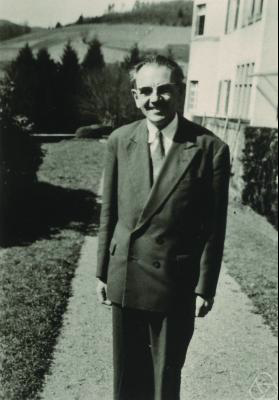
\includegraphics[width=0.52cm,height=0.62cm,keepaspectratio]{images/Leray.png}
      };
      \node[inner sep=0pt] at (-3.77,1.02) {
        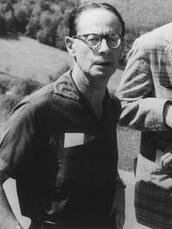
\includegraphics[width=0.52cm,height=0.62cm,keepaspectratio]{images/Weil.png}
      };
      \node[inner sep=0pt] at (-3.19,1.02) {
        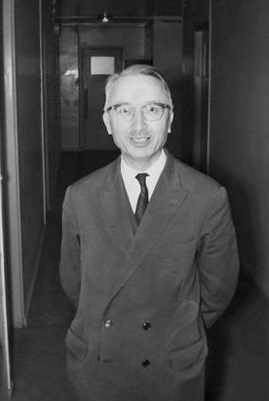
\includegraphics[width=0.52cm,height=0.62cm,keepaspectratio]{images/Cartan.png}
      };
      \node[inner sep=0pt] at (-2.61,1.02) {
        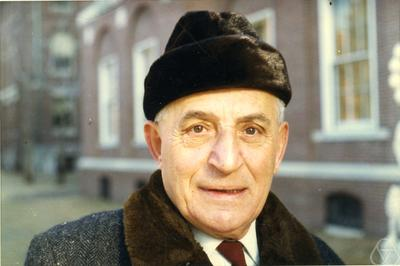
\includegraphics[width=0.52cm,height=0.62cm,keepaspectratio]{images/Zariski.jpg}
      };
      \node[inner sep=0pt] at (-2.03,1.02) {
        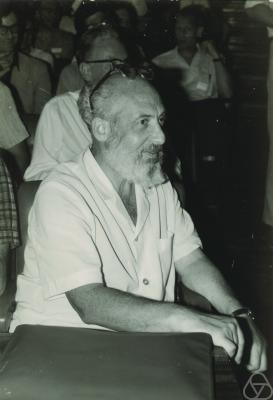
\includegraphics[width=0.52cm,height=0.62cm,keepaspectratio]{images/Eilenberg.jpg}
      };
      \node[inner sep=0pt] at (-1.45,1.02) {
        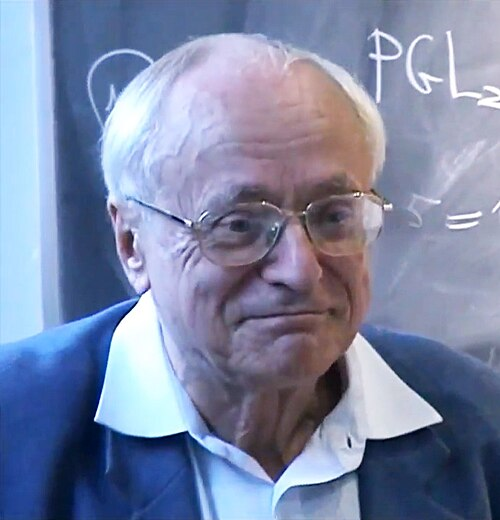
\includegraphics[width=0.52cm,height=0.62cm,keepaspectratio]{images/Serre.jpg}
      };
      \node[inner sep=0pt] at (-0.87,1.02) {
        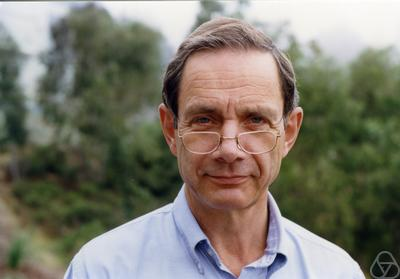
\includegraphics[width=0.52cm,height=0.62cm,keepaspectratio]{images/Artin.jpg}
      };
      \node[inner sep=0pt] at (-0.29,1.02) {
        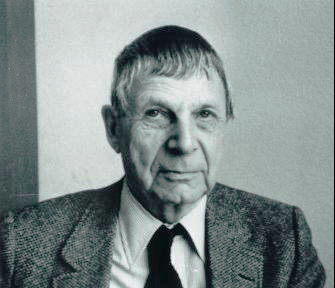
\includegraphics[width=0.52cm,height=0.62cm,keepaspectratio]{images/Ahlfors.png}
      };
      \node[inner sep=0pt] at (0.29,1.02) {
        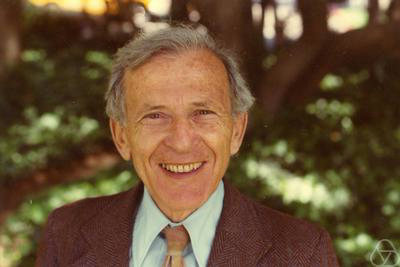
\includegraphics[width=0.52cm,height=0.62cm,keepaspectratio]{images/Lewy.png}
      };
      \node[inner sep=0pt] at (0.87,1.02) {
        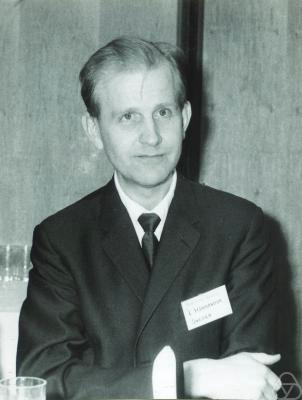
\includegraphics[width=0.52cm,height=0.62cm,keepaspectratio]{images/Hormander.png}
      };
      \node[inner sep=0pt] at (1.45,1.02) {
        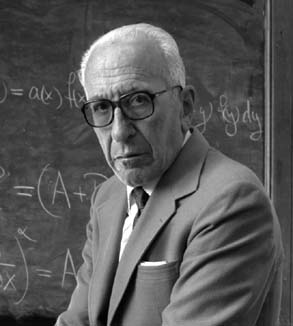
\includegraphics[width=0.52cm,height=0.62cm,keepaspectratio]{images/Calderon.png}
      };
      \node[inner sep=0pt] at (2.03,1.02) {
        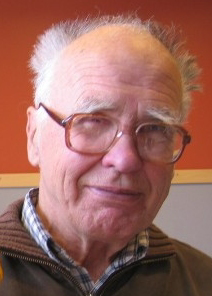
\includegraphics[width=0.52cm,height=0.62cm,keepaspectratio]{images/Carleson.png}
      };
      \node[inner sep=0pt] at (2.61,1.02) {
        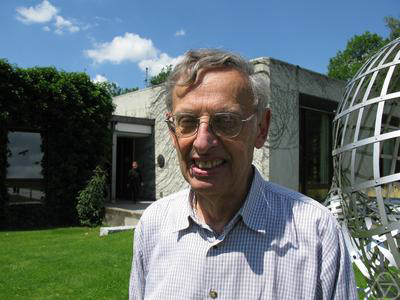
\includegraphics[width=0.52cm,height=0.62cm,keepaspectratio]{images/Stein.png}
      };
      \node[inner sep=0pt] at (3.19,1.02) {
        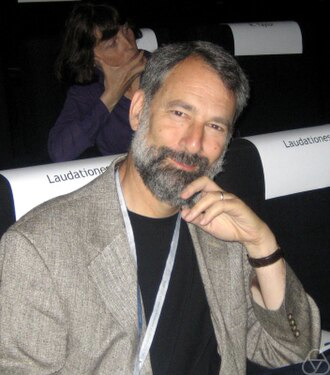
\includegraphics[width=0.52cm,height=0.62cm,keepaspectratio]{images/Fefferman.png}
      };
      \node[inner sep=0pt] at (3.77,1.02) {
        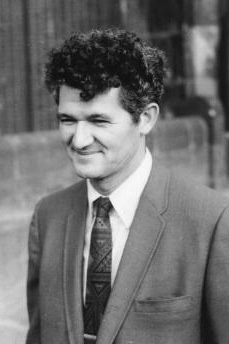
\includegraphics[width=0.52cm,height=0.62cm,keepaspectratio]{images/Lax.jpg}
      };
      \node[inner sep=0pt] at (4.35,1.02) {
        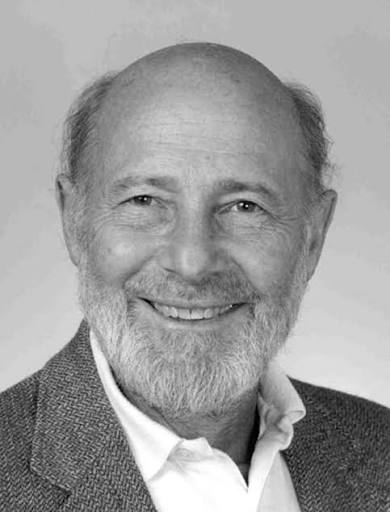
\includegraphics[width=0.52cm,height=0.62cm,keepaspectratio]{images/Keller.jpg}
      };
      \node[inner sep=0pt] at (-4.35,0.34) {
        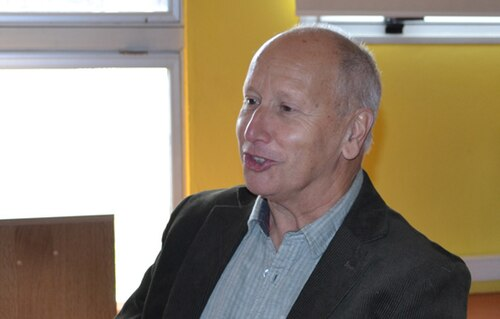
\includegraphics[width=0.52cm,height=0.62cm,keepaspectratio]{images/Caffarelli.jpg}
      };
      \node[inner sep=0pt] at (-3.77,0.34) {
        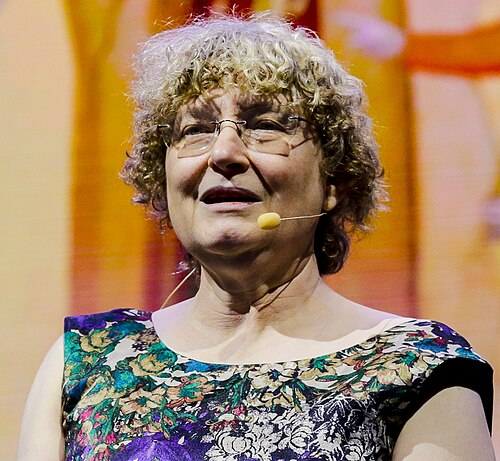
\includegraphics[width=0.52cm,height=0.62cm,keepaspectratio]{images/Daubechies.jpg}
      };
      \node[inner sep=0pt] at (-3.19,0.34) {
        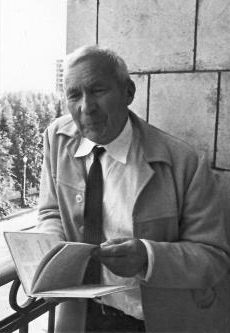
\includegraphics[width=0.52cm,height=0.62cm,keepaspectratio]{images/Kolmogorov.jpg}
      };
      \node[inner sep=0pt] at (-2.61,0.34) {
        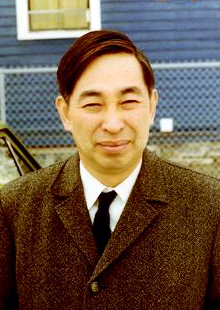
\includegraphics[width=0.52cm,height=0.62cm,keepaspectratio]{images/Ito.jpg}
      };
      \node[inner sep=0pt] at (-2.03,0.34) {
        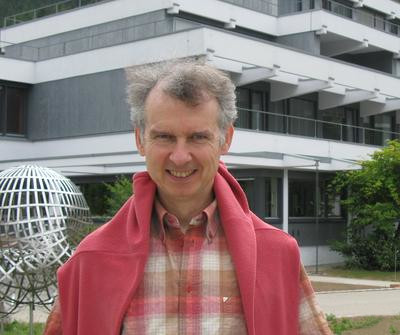
\includegraphics[width=0.52cm,height=0.62cm,keepaspectratio]{images/LeGall.jpg}
      };
      \node[inner sep=0pt] at (-1.45,0.34) {
        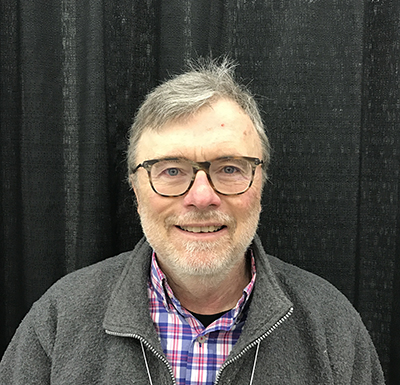
\includegraphics[width=0.52cm,height=0.62cm,keepaspectratio]{images/Gregory-Lawler-2019.jpg}
      };
      \node[inner sep=0pt] at (-0.87,0.34) {
        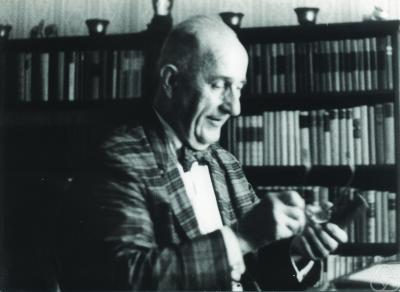
\includegraphics[width=0.52cm,height=0.62cm,keepaspectratio]{images/Siegel.jpeg}
      };
      \node[inner sep=0pt] at (-0.29,0.34) {
        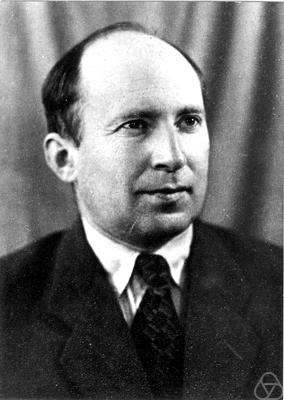
\includegraphics[width=0.52cm,height=0.62cm,keepaspectratio]{images/Gelfand.jpg}
      };
      \node[inner sep=0pt] at (0.29,0.34) {
        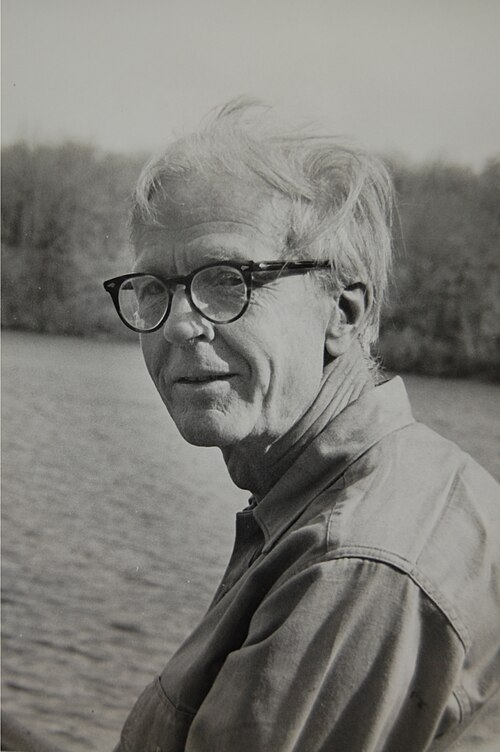
\includegraphics[width=0.52cm,height=0.62cm,keepaspectratio]{images/Whitney.jpg}
      };
      \node[inner sep=0pt] at (0.87,0.34) {
        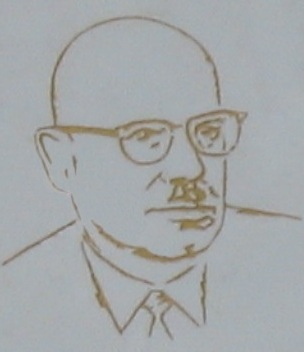
\includegraphics[width=0.52cm,height=0.62cm,keepaspectratio]{images/Krein.jpg}
      };
      \node[inner sep=0pt] at (1.45,0.34) {
        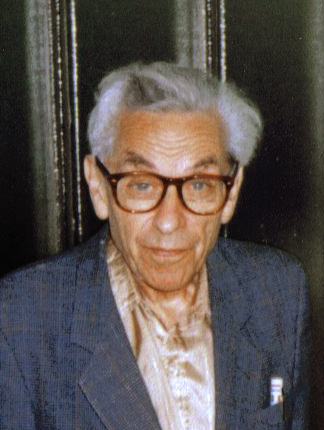
\includegraphics[width=0.52cm,height=0.62cm,keepaspectratio]{images/Erdos.jpg}
      };
      \node[inner sep=0pt] at (2.03,0.34) {
        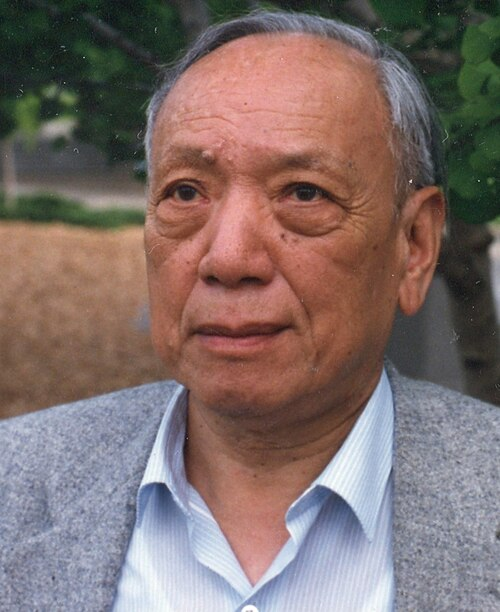
\includegraphics[width=0.52cm,height=0.62cm,keepaspectratio]{images/Chern.jpg}
      };
      \node[inner sep=0pt] at (2.61,0.34) {
        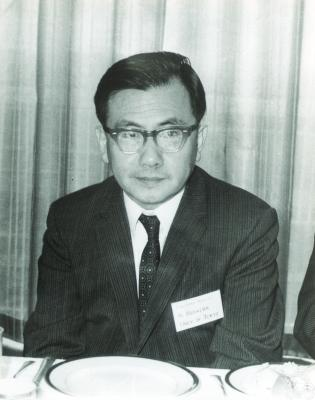
\includegraphics[width=0.52cm,height=0.62cm,keepaspectratio]{images/Kodaira.jpg}
      };
      \node[inner sep=0pt] at (3.19,0.34) {
        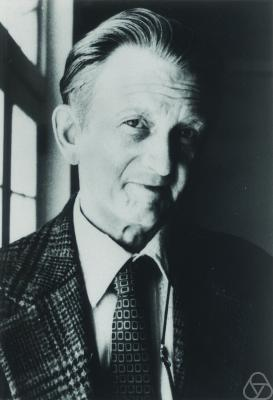
\includegraphics[width=0.52cm,height=0.62cm,keepaspectratio]{images/Selberg.jpg}
      };
      \node[inner sep=0pt] at (3.77,0.34) {
        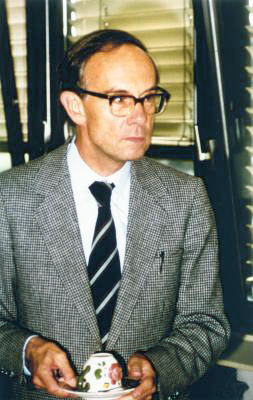
\includegraphics[width=0.52cm,height=0.62cm,keepaspectratio]{images/Hirzebruch.jpeg}
      };
      \node[inner sep=0pt] at (4.35,0.34) {
        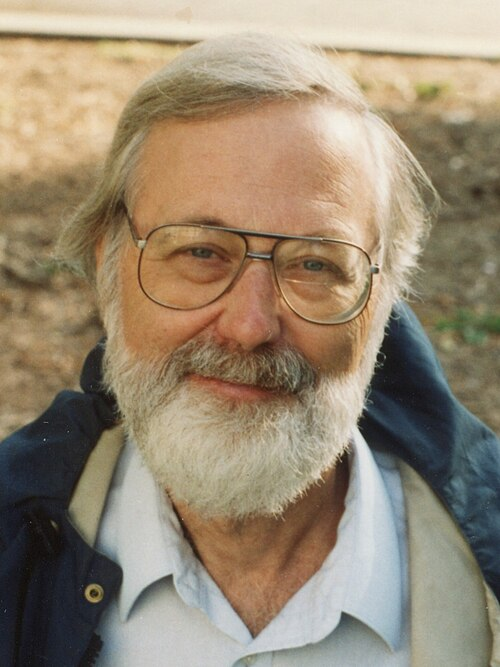
\includegraphics[width=0.52cm,height=0.62cm,keepaspectratio]{images/Milnor.jpg}
      };
      \node[inner sep=0pt] at (-4.35,-0.34) {
        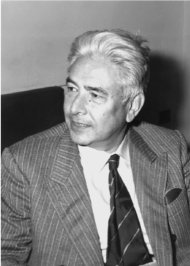
\includegraphics[width=0.52cm,height=0.62cm,keepaspectratio]{images/DeGiorgi.jpg}
      };
      \node[inner sep=0pt] at (-3.77,-0.34) {
        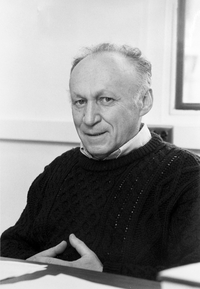
\includegraphics[width=0.52cm,height=0.62cm,keepaspectratio]{images/PiatetskiShapiro.jpg}
      };
      \node[inner sep=0pt] at (-3.19,-0.34) {
        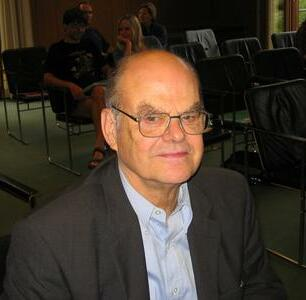
\includegraphics[width=0.52cm,height=0.62cm,keepaspectratio]{images/Thompson.jpg}
      };
      \node[inner sep=0pt] at (-2.61,-0.34) {
        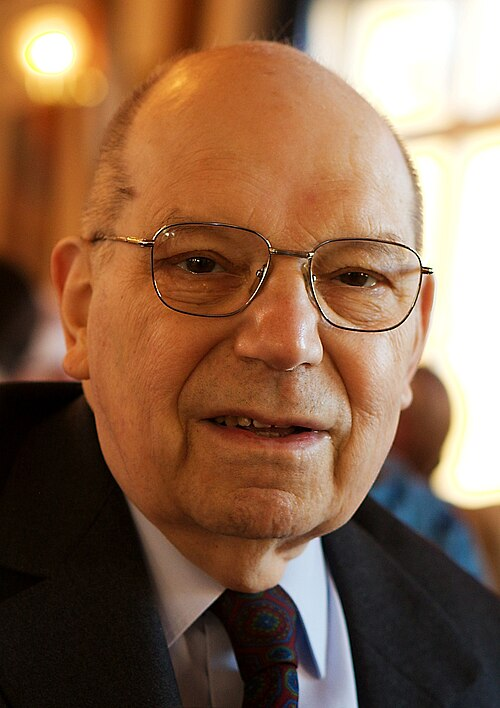
\includegraphics[width=0.52cm,height=0.62cm,keepaspectratio]{images/Tits.jpg}
      };
      \node[inner sep=0pt] at (-2.03,-0.34) {
        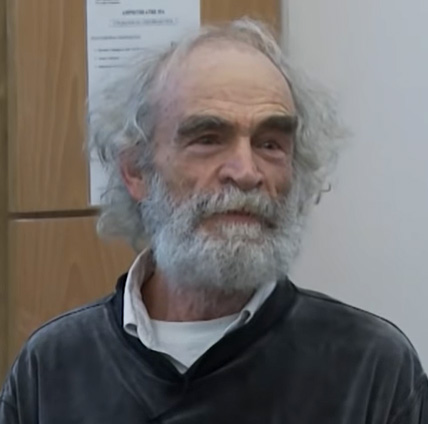
\includegraphics[width=0.52cm,height=0.62cm,keepaspectratio]{images/Gromov.jpg}
      };
      \node[inner sep=0pt] at (-1.45,-0.34) {
        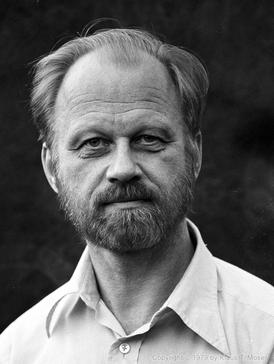
\includegraphics[width=0.52cm,height=0.62cm,keepaspectratio]{images/Moser.jpg}
      };
      \node[inner sep=0pt] at (-0.87,-0.34) {
        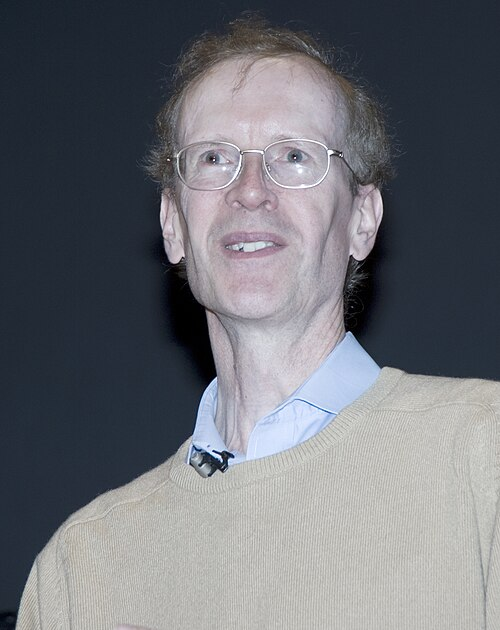
\includegraphics[width=0.52cm,height=0.62cm,keepaspectratio]{images/Wiles.jpg}
      };
      \node[inner sep=0pt] at (-0.29,-0.34) {
        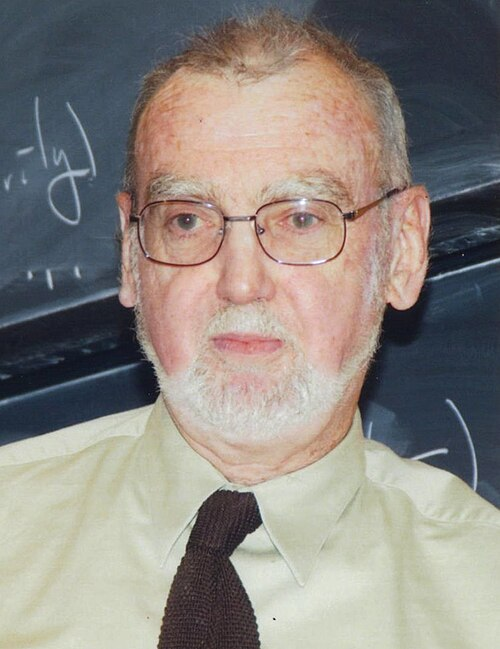
\includegraphics[width=0.52cm,height=0.62cm,keepaspectratio]{images/Langlands.jpg}
      };
      \node[inner sep=0pt] at (0.29,-0.34) {
        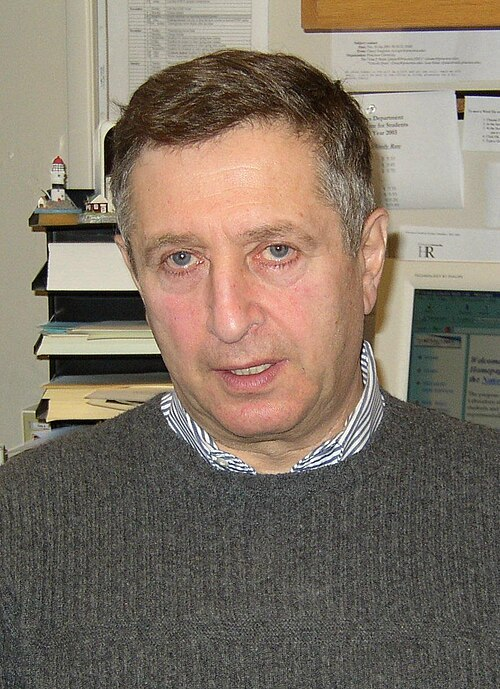
\includegraphics[width=0.52cm,height=0.62cm,keepaspectratio]{images/Sinai.jpg}
      };
      \node[inner sep=0pt] at (0.87,-0.34) {
        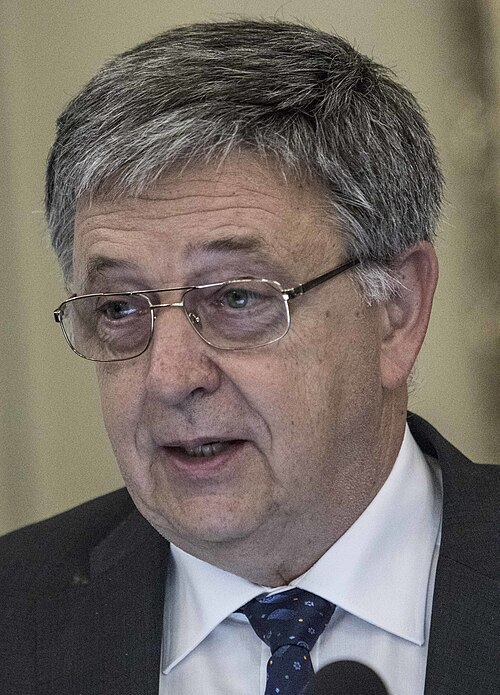
\includegraphics[width=0.52cm,height=0.62cm,keepaspectratio]{images/Lovasz.jpg}
      };
      \node[inner sep=0pt] at (1.45,-0.34) {
        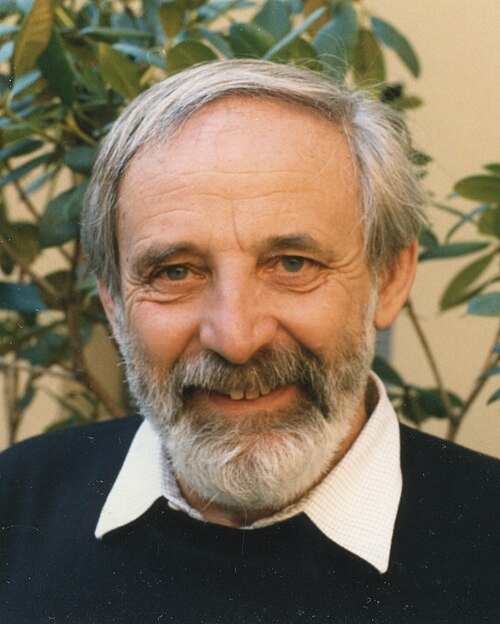
\includegraphics[width=0.52cm,height=0.62cm,keepaspectratio]{images/Bott.jpg}
      };
      \node[inner sep=0pt] at (2.03,-0.34) {
        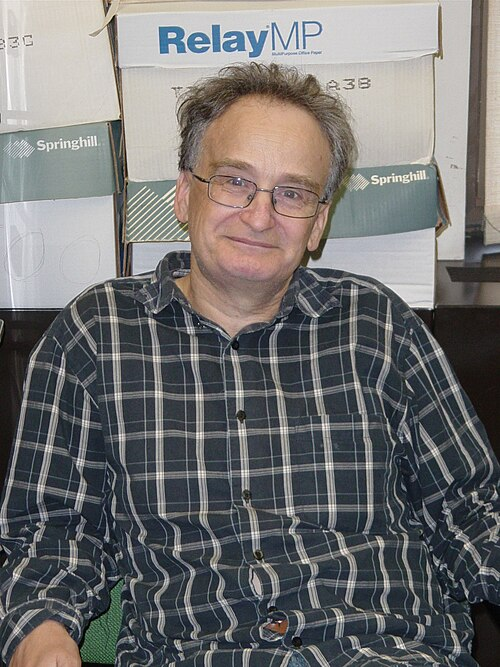
\includegraphics[width=0.52cm,height=0.62cm,keepaspectratio]{images/Shelah.jpg}
      };
      \node[inner sep=0pt] at (2.61,-0.34) {
        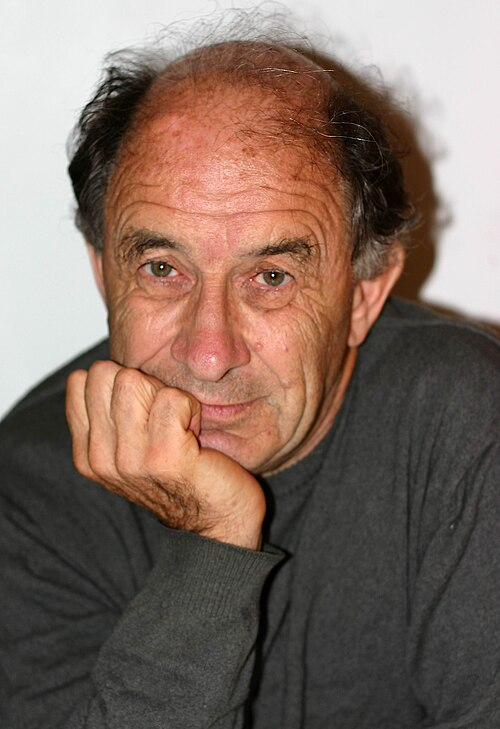
\includegraphics[width=0.52cm,height=0.62cm,keepaspectratio]{images/Arnold.jpg}
      };
      \node[inner sep=0pt] at (3.19,-0.34) {
        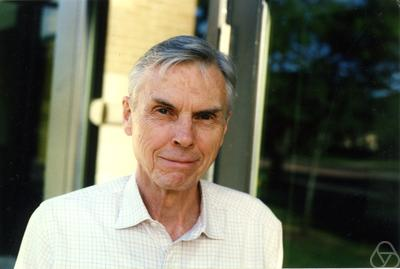
\includegraphics[width=0.52cm,height=0.62cm,keepaspectratio]{images/Tate.jpg}
      };
      \node[inner sep=0pt] at (3.77,-0.34) {
        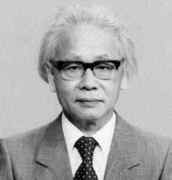
\includegraphics[width=0.52cm,height=0.62cm,keepaspectratio]{images/Mikio_Sato.jpg}
      };
      \node[inner sep=0pt] at (4.35,-0.34) {
        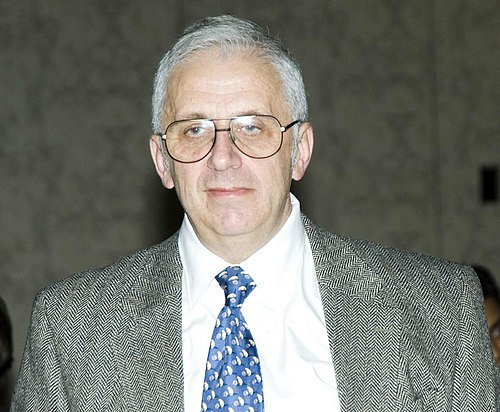
\includegraphics[width=0.52cm,height=0.62cm,keepaspectratio]{images/Margulis.jpg}
      };
      \node[inner sep=0pt] at (-4.35,-1.02) {
        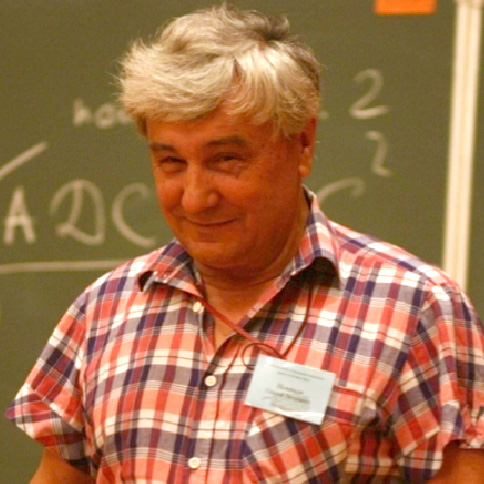
\includegraphics[width=0.52cm,height=0.62cm,keepaspectratio]{images/Novikov.jpg}
      };
      \node[inner sep=0pt] at (-3.77,-1.02) {
        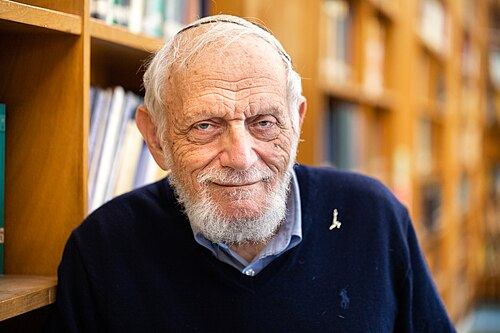
\includegraphics[width=0.52cm,height=0.62cm,keepaspectratio]{images/Furstenberg.jpg}
      };
      \node[inner sep=0pt] at (-3.19,-1.02) {
        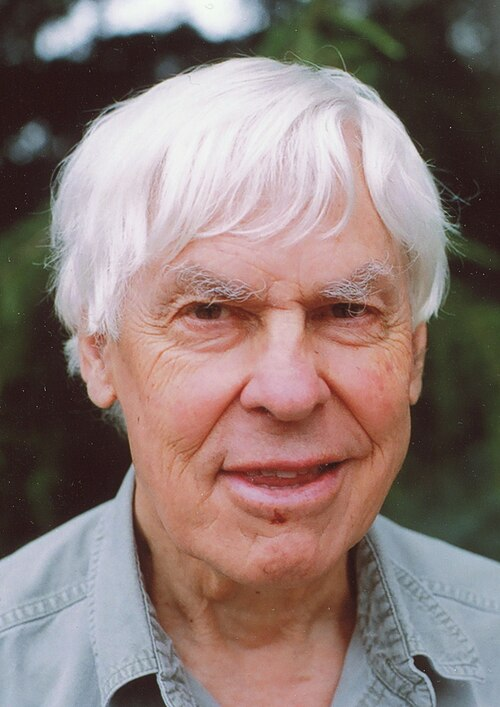
\includegraphics[width=0.52cm,height=0.62cm,keepaspectratio]{images/Smale.jpg}
      };
      \node[inner sep=0pt] at (-2.61,-1.02) {
        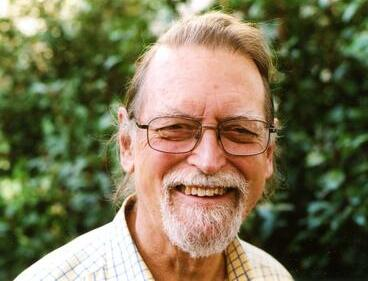
\includegraphics[width=0.52cm,height=0.62cm,keepaspectratio]{images/Mumford.jpg}
      };
      \node[inner sep=0pt] at (-2.03,-1.02) {
        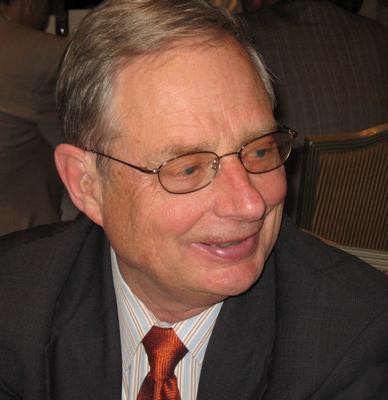
\includegraphics[width=0.52cm,height=0.62cm,keepaspectratio]{images/Griffiths.jpeg}
      };
      \node[inner sep=0pt] at (-1.45,-1.02) {
        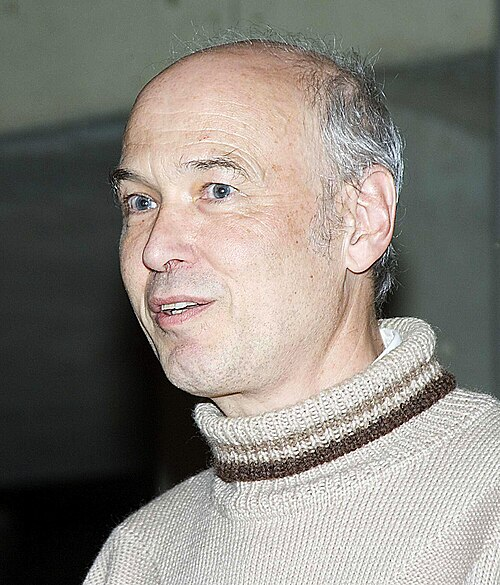
\includegraphics[width=0.52cm,height=0.62cm,keepaspectratio]{images/Deligne.jpg}
      };
      \node[inner sep=0pt] at (-0.87,-1.02) {
        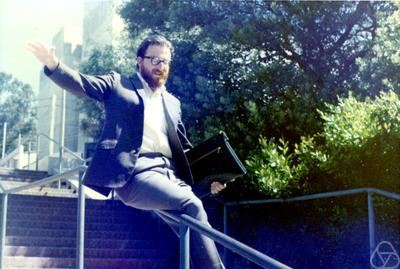
\includegraphics[width=0.52cm,height=0.62cm,keepaspectratio]{images/Sullivan.jpg}
      };
      \node[inner sep=0pt] at (-0.29,-1.02) {
        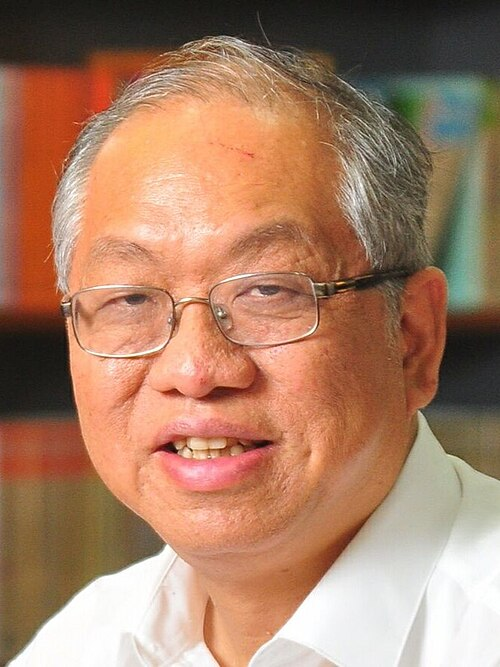
\includegraphics[width=0.52cm,height=0.62cm,keepaspectratio]{images/Yau.jpg}
      };
      \node[inner sep=0pt] at (0.29,-1.02) {
        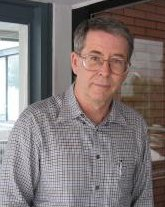
\includegraphics[width=0.52cm,height=0.62cm,keepaspectratio]{images/Aschbacher.jpg}
      };
      \node[inner sep=0pt] at (0.87,-1.02) {
        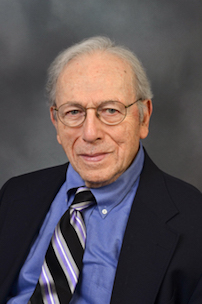
\includegraphics[width=0.52cm,height=0.62cm,keepaspectratio]{images/Mostow.jpg}
      };
      \node[inner sep=0pt] at (1.45,-1.02) {
        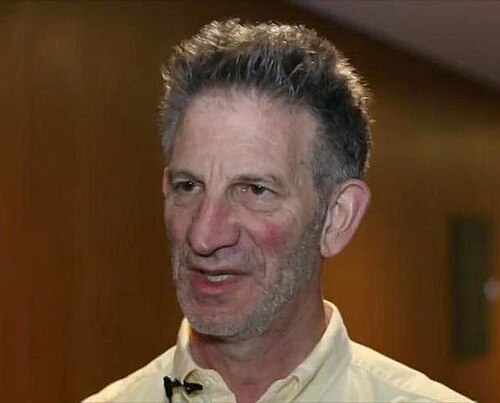
\includegraphics[width=0.52cm,height=0.62cm,keepaspectratio]{images/Sarnak.jpg}
      };
      \node[inner sep=0pt] at (2.03,-1.02) {
        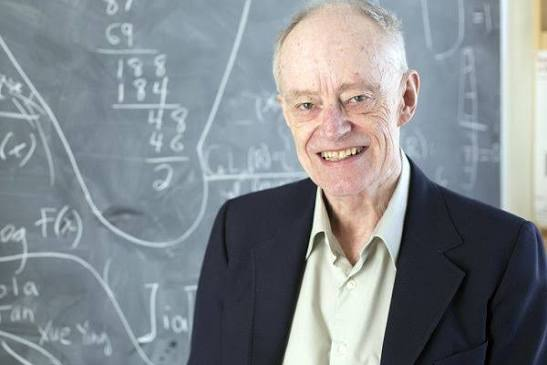
\includegraphics[width=0.52cm,height=0.62cm,keepaspectratio]{images/Arthur.jpeg}
      };
      \node[inner sep=0pt] at (2.61,-1.02) {
        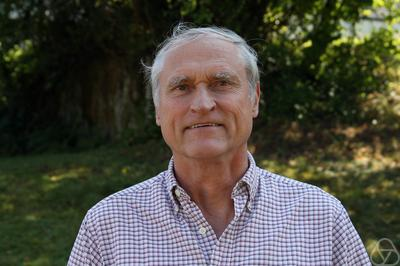
\includegraphics[width=0.52cm,height=0.62cm,keepaspectratio]{images/Schoen.jpg}
      };
      \node[inner sep=0pt] at (3.19,-1.02) {
        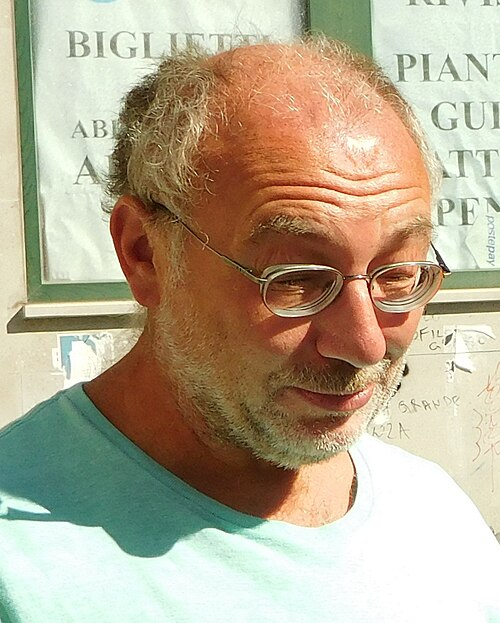
\includegraphics[width=0.52cm,height=0.62cm,keepaspectratio]{images/Beilinson.jpg}
      };
      \node[inner sep=0pt] at (3.77,-1.02) {
        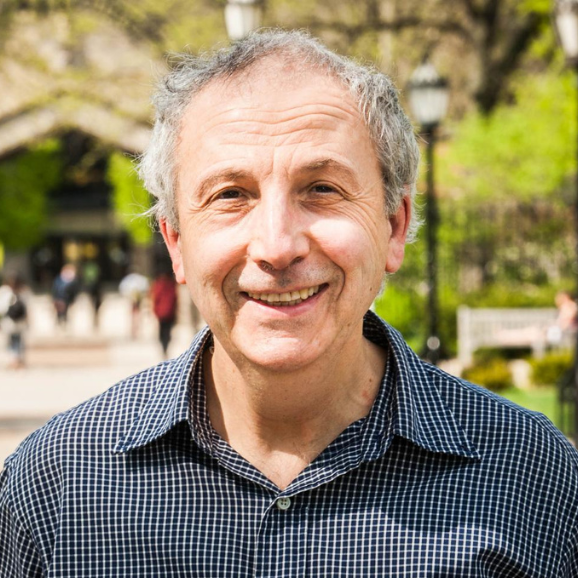
\includegraphics[width=0.52cm,height=0.62cm,keepaspectratio]{images/Vladimir_Drinfeld.png}
      };
      \node[inner sep=0pt] at (4.35,-1.02) {
        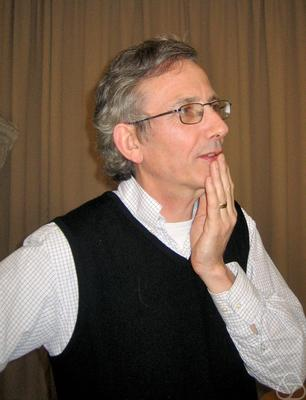
\includegraphics[width=0.52cm,height=0.62cm,keepaspectratio]{images/Donaldson.jpg}
      };
    \end{tikzpicture}
  };
  \node[anchor=south, font=\scriptsize, text=coverdark!40]
    at ([yshift=0.38cm]current page.south) {\faIcon{medal}\enspace Wolf Prize in Mathematics\enspace|\enspace 合集\enspace|\enspace 人物谱系};
\end{tikzpicture}
\end{frame}
}

% ---- Full-page chapter divider: #1 number #2 title #3 subtitle ----
\newcommand{\chapterdivider}[3]{%
\begin{frame}[plain]
\begin{tikzpicture}[remember picture, overlay]
  \fill[coverdark] (current page.north west) rectangle (current page.south east);
  \fill[coverprimary!30, opacity=0.35] (current page.north west) ++(2.0,-1.6) circle (2.6cm);
  \fill[coveraccent!30, opacity=0.30] (current page.south east) ++(-2.2,1.7) circle (2.9cm);
  \node[anchor=center, font=\fontsize{15}{19}\selectfont\bfseries, text=coveraccent!85]
    at ([yshift=1.9cm]current page.center) {#1};
  \node[anchor=center, font=\fontsize{23}{29}\selectfont\bfseries, text=white]
    at ([yshift=0.7cm]current page.center) {#2};
  \draw[coveraccent!70, line width=1.2pt] ([yshift=-0.15cm, xshift=-5.2cm]current page.center)
    -- ([yshift=-0.15cm, xshift=5.2cm]current page.center);
  \node[anchor=center, font=\fontsize{11}{14}\selectfont, text=coverlight]
    at ([yshift=-0.95cm]current page.center) {#3};
\end{tikzpicture}
\end{frame}
}
% ===== 得主宏 =====
\newcommand{\lerayslide}{%
\personslideA
  {Jean Leray}
  {让·勒雷：层论与谱序列的发明者}
{images/Leray.png}
  {Photo: Wikipedia}
  {1979（73岁）}
  {1906--1998（享年92岁）}
  {法国}
  {Collège de France}
  {Leray 在战俘营中发展出层（sheaf）、谱序列与拓扑度理论，为代数拓扑和偏微分方程提供了全新工具，深刻影响了 Cartan、Serre 等一代法国数学家。\\[3pt]
  \textbf{一句话：} 一个在极端环境中诞生的抽象工具，后来成为整个现代几何与拓扑的通用语言。}
}
\newcommand{\weilslide}{%
\personslideA
  {André Weil}
  {安德烈·韦伊：现代代数几何与 Bourbaki 的核心}
{images/Weil.png}
  {Photo: Wikipedia}
  {1979（73岁）}
  {1906--1998（享年92岁）}
  {法国}
  {Institute for Advanced Study}
  {Weil 重建了代数几何的基础，提出著名的 Weil 猜想连接数论与拓扑，并作为 Bourbaki 学派核心推动了数学的公理化重写。\\[3pt]
  \textbf{一句话：} 层论与代数几何这两条主线，从 Leray 与 Weil 起步，贯穿本集其后每一位得主。}
}
\newcommand{\cartanslide}{%
\personslideA
  {Henri Cartan}
  {亨利·嘉当：同调代数与层论的组织者}
{images/Cartan.png}
  {Photo: Wikipedia}
  {1980（76岁）}
  {1904--2008（享年104岁）}
  {法国}
  {Université Paris-Sud}
  {Cartan 是 Bourbaki 创始成员，主持著名的"Cartan 讨论班"，与 Eilenberg 合著《同调代数》，在多复变、层论和 Steenrod 代数上贡献广泛，培养了 Serre 等一代法国数学家。\\[3pt]
  \textbf{一句话：} 他把层与同调代数组织成可教、可用的体系，是这场抽象化运动的枢纽人物。}
}
\newcommand{\zariskislide}{%
\personslideA
  {Oscar Zariski}
  {奥斯卡·扎里斯基：用交换代数重铸代数几何}
{images/Zariski.jpg}
  {Photo: Wikipedia}
  {1981（82岁）}
  {1899--1986（享年87岁）}
  {美国（意大利裔）}
  {Harvard University}
  {Zariski 把严格的交换代数方法引入代数几何，澄清了意大利学派的直观论证，创立 Zariski 拓扑与 Zariski 主定理，为现代代数几何奠定坚实地基。\\[3pt]
  \textbf{一句话：} 他让代数几何从"看得见的直觉"变成"证得出的结构"，直接铺就概型理论之路。}
}
\newcommand{\eilenbergslide}{%
\personslideA
  {Samuel Eilenberg}
  {萨缪尔·艾伦伯格：范畴论的共同创立者}
{images/Eilenberg.jpg}
  {Photo: Wikipedia}
  {1986（73岁）}
  {1913--1998（享年85岁）}
  {美国（波兰裔）}
  {Columbia University}
  {Eilenberg 与 Mac Lane 共同创立范畴论，引入函子与自然变换；与 Cartan 合著《同调代数》，并奠定代数拓扑的公理化基础（Eilenberg-Steenrod 公理）。\\[3pt]
  \textbf{一句话：} 他提供了"对象之间的映射"这一视角，成为整个现代数学的通用语法。}
}
\newcommand{\serreslide}{%
\def\crosscontent{\vspace{3pt}
  \begin{tikzpicture}
    \node[draw=coveraccent!45, fill=panel!60, rounded corners=3pt, inner xsep=5pt, inner ysep=4pt, text width=3.8cm, align=left] {
      {\fontsize{6}{7}\selectfont\bfseries\color{coveraccent!65!black} $\blacklozenge$ 菲尔兹奖}\enspace{\fontsize{6}{7}\selectfont\color{coverdark!80} 1954（27岁）}\\[1.5pt]{\fontsize{6}{7}\selectfont\bfseries\color{coveraccent!65!black} $\blacktriangle$ 阿贝尔奖}\enspace{\fontsize{6}{7}\selectfont\color{coverdark!80} 2003（77岁）}
    };
  \end{tikzpicture}}
\personslideA
  {Jean-Pierre Serre}
  {让-皮埃尔·塞尔：现代数学的多面奠基人}
{images/Serre.jpg}
  {Photo: Wikipedia}
  {2000（74岁）}
  {1926--}
  {法国}
  {Collège de France}
  {Serre 把层与上同调引入代数几何（FAC/GAGA），在代数拓扑、数论与表示论都留下核心工作，直接启发 Grothendieck 的概型理论。他是首位同获菲尔兹奖、阿贝尔奖与沃尔夫奖的数学家。\\[3pt]
  \textbf{一句话：} 从拓扑到数论，他反复用"层"这把钥匙打开新的领域。}
}
\newcommand{\artinslide}{%
\personslideA
  {Michael Artin}
  {迈克尔·阿廷：把概型语言推向新高度}
{images/Artin.jpg}
  {Photo: Wikipedia}
  {2013（79岁）}
  {1934--}
  {美国}
  {MIT}
  {Artin 是 Grothendieck 概型纲领的关键合作者，发展 étale 上同调、代数空间与代数层叠（stack），并在非交换环上做出深刻工作。他是数论学家 Emil Artin 之子。\\[3pt]
  \textbf{一句话：} 他把 Serre 与 Grothendieck 打下的地基继续扩建，让代数几何能容纳更一般的几何对象。}
}
\newcommand{\ahlforsslide}{%
\def\crosscontent{\vspace{3pt}
  \begin{tikzpicture}
    \node[draw=coveraccent!45, fill=panel!60, rounded corners=3pt, inner xsep=5pt, inner ysep=4pt, text width=3.8cm, align=left] {
      {\fontsize{6}{7}\selectfont\bfseries\color{coveraccent!65!black} $\blacklozenge$ 菲尔兹奖}\enspace{\fontsize{6}{7}\selectfont\color{coverdark!80} 1936（29岁）}
    };
  \end{tikzpicture}}
\personslideA
  {Lars Ahlfors}
  {拉尔斯·阿尔福斯：黎曼曲面与复分析的几何化}
{images/Ahlfors.png}
  {Photo: Wikipedia}
  {1981（74岁）}
  {1907--1996（享年89岁）}
  {芬兰/美国}
  {Harvard University}
  {Ahlfors 在黎曼曲面、拟共形映射与复分析上贡献深刻。他是 1936 年首届菲尔兹奖得主，也是首位同时拿下菲尔兹奖与沃尔夫奖的数学家。\\[3pt]
  \textbf{一句话：} 复分析不是"会算积分"的技巧，而是一种描述空间结构的几何语言。}
}
\newcommand{\lewyslide}{%
\personslideA
  {Hans Lewy}
  {汉斯·莱维：揭示偏微分方程的意外}
{images/Lewy.png}
  {Photo: Wikipedia}
  {1984/85（80岁）}
  {1904--1988（享年84岁）}
  {美国（德国裔）}
  {UC Berkeley}
  {Lewy 在偏微分方程、极小曲面与多复变上贡献突出，最著名的是构造出"没有任何解"的光滑线性 PDE（Lewy 例子），彻底改变了人们对方程可解性的认识。\\[3pt]
  \textbf{一句话：} 有些方程再光滑也无解——这个反例告诉数学家，可解性本身就是深刻的问题。}
}
\newcommand{\hormanderslide}{%
\def\crosscontent{\vspace{3pt}
  \begin{tikzpicture}
    \node[draw=coveraccent!45, fill=panel!60, rounded corners=3pt, inner xsep=5pt, inner ysep=4pt, text width=3.8cm, align=left] {
      {\fontsize{6}{7}\selectfont\bfseries\color{coveraccent!65!black} $\blacklozenge$ 菲尔兹奖}\enspace{\fontsize{6}{7}\selectfont\color{coverdark!80} 1962（31岁）}
    };
  \end{tikzpicture}}
\personslideA
  {Lars Hörmander}
  {拉尔斯·赫尔曼德尔：线性偏微分算子的总设计师}
{images/Hormander.png}
  {Photo: Wikipedia}
  {1988（57岁）}
  {1931--2012（享年81岁）}
  {瑞典}
  {Lund University}
  {Hörmander 建立线性偏微分算子的一般理论，奠定微局部分析。他 1962 年获菲尔兹奖，四卷本《线性偏微分算子分析》是该领域的圣经。\\[3pt]
  \textbf{一句话：} 他解释了奇异性如何在方程里运动，让 PDE 的"何时有解、解多光滑"变成可计算的问题。}
}
\newcommand{\calderonslide}{%
\personslideA
  {Alberto Calderón}
  {阿尔贝托·卡尔德龙：奇异积分理论的奠基者}
{images/Calderon.png}
  {Photo: Wikipedia}
  {1989（69岁）}
  {1920--1998（享年78岁）}
  {阿根廷/美国}
  {University of Chicago}
  {Calderón 与 Zygmund 创立 Calderón-Zygmund 奇异积分理论，深刻推进偏微分方程与调和分析。他领导的芝加哥学派培养了大批分析学家。\\[3pt]
  \textbf{一句话：} 奇异积分是分析学的"手术刀"，让数学家能精确处理带奇点的算子与方程。}
}
\newcommand{\carlesonslide}{%
\def\crosscontent{\vspace{3pt}
  \begin{tikzpicture}
    \node[draw=coveraccent!45, fill=panel!60, rounded corners=3pt, inner xsep=5pt, inner ysep=4pt, text width=3.8cm, align=left] {
      {\fontsize{6}{7}\selectfont\bfseries\color{coveraccent!65!black} $\blacktriangle$ 阿贝尔奖}\enspace{\fontsize{6}{7}\selectfont\color{coverdark!80} 2006（78岁）}
    };
  \end{tikzpicture}}
\personslideA
  {Lennart Carleson}
  {伦纳特·卡尔松：攻克 Fourier 级数收敛}
{images/Carleson.png}
  {Photo: Wikipedia}
  {1992（64岁）}
  {1928--}
  {瑞典}
  {Uppsala University / UCLA}
  {Carleson 证明平方可积函数的 Fourier 级数几乎处处收敛（Carleson 定理），解决了悬置半个多世纪的 Lusin 猜想，并提出 Carleson 测度等核心工具。他是 2006 年阿贝尔奖得主。\\[3pt]
  \textbf{一句话：} 他给出了 Fourier 分析最深的"极限之问"的答案。}
}
\newcommand{\steinslide}{%
\personslideA
  {Elias M. Stein}
  {伊莱亚斯·斯坦因：现代调和分析的宗师}
{images/Stein.png}
  {Photo: Wikipedia}
  {1999（68岁）}
  {1931--2018（享年87岁）}
  {美国}
  {Princeton University}
  {Stein 在奇异积分、Hardy 空间与多参数分析上做出奠基性工作，重塑了现代调和分析。他培养了包括 Fefferman、Tao 在内的多位菲尔兹奖得主。\\[3pt]
  \textbf{一句话：} 他不仅推进了理论，还教出了一整个学派，把调和分析变成通向多个领域的桥梁。}
}
\newcommand{\feffermanslide}{%
\def\crosscontent{\vspace{3pt}
  \begin{tikzpicture}
    \node[draw=coveraccent!45, fill=panel!60, rounded corners=3pt, inner xsep=5pt, inner ysep=4pt, text width=3.8cm, align=left] {
      {\fontsize{6}{7}\selectfont\bfseries\color{coveraccent!65!black} $\blacklozenge$ 菲尔兹奖}\enspace{\fontsize{6}{7}\selectfont\color{coverdark!80} 1978（29岁）}
    };
  \end{tikzpicture}}
\personslideA
  {Charles Fefferman}
  {查尔斯·费弗曼：多复变与调和分析的天才}
{images/Fefferman.png}
  {Photo: Wikipedia}
  {2017（68岁）}
  {1949--}
  {美国}
  {Princeton University}
  {Fefferman 在调和分析、多复变函数与偏微分方程上贡献卓著，如 BMO 与 Hardy 空间对偶、复域的 Bergman 核分析。他 1978 年获菲尔兹奖，是 Stein 的学生。\\[3pt]
  \textbf{一句话：} 本集以他收束：调和分析成为贯通复分析、PDE 与几何的现代语言。}
}
\newcommand{\laxslide}{%
\def\crosscontent{\vspace{3pt}
  \begin{tikzpicture}
    \node[draw=coveraccent!45, fill=panel!60, rounded corners=3pt, inner xsep=5pt, inner ysep=4pt, text width=3.8cm, align=left] {
      {\fontsize{6}{7}\selectfont\bfseries\color{coveraccent!65!black} $\blacktriangle$ 阿贝尔奖}\enspace{\fontsize{6}{7}\selectfont\color{coverdark!80} 2005（79岁）}
    };
  \end{tikzpicture}}
\personslide
  {Peter Lax}
  {彼得·拉克斯：PDE、守恒律与计算数学的桥梁}
  {\portraitbox{images/Lax.jpg}{Photo: Wikipedia}}
  {1987（61岁）}
  {1926--}
  {匈牙利/美国}
  {Courant Institute, NYU}
  {Lax 在偏微分方程、散射理论、双曲守恒律、数值分析和数学物理中贡献深远；Lax 对、Lax-Milgram 定理、Lax 等价定理等名字贯穿现代分析与计算。2005 年获阿贝尔奖。}
  {他把 PDE 从黑板上的理论，推进为理解物理和计算世界的共同语言。}
}
\newcommand{\kellerslide}{%
\personslide
  {Joseph B. Keller}
  {约瑟夫·凯勒：渐近方法与几何绕射理论}
  {\portraitbox{images/Keller.jpg}{Photo: MacTutor}}
  {1996/97（73岁）}
  {1923--2016（享年93岁）}
  {美国}
  {Stanford University}
  {Keller 专长应用数学，最著名的是几何绕射理论；他还研究波传播、量子系统的 EBK 方法、非反射边界条件、流体和工程问题。1988 年获美国国家科学奖章。}
  {他让近似计算成为理解真实波动现象的精密工具。}
}
\newcommand{\caffarellislide}{%
\def\crosscontent{\vspace{3pt}
  \begin{tikzpicture}
    \node[draw=coveraccent!45, fill=panel!60, rounded corners=3pt, inner xsep=5pt, inner ysep=4pt, text width=3.8cm, align=left] {
      {\fontsize{6}{7}\selectfont\bfseries\color{coveraccent!65!black} $\blacktriangle$ 阿贝尔奖}\enspace{\fontsize{6}{7}\selectfont\color{coverdark!80} 2023（75岁）}
    };
  \end{tikzpicture}}
\personslide
  {Luis Caffarelli}
  {路易斯·卡法雷利：非线性 PDE 与自由边界}
  {\portraitbox{images/Caffarelli.jpg}{Photo: Wikipedia}}
  {2012（63岁）}
  {1948--}
  {阿根廷/美国}
  {University of Texas at Austin}
  {Caffarelli 在非线性偏微分方程、自由边界问题、正则性理论与 Monge-Ampere 方程上做出奠基性贡献；2023 年获阿贝尔奖，表彰其在非线性 PDE 正则性理论中的开创作用。}
  {他研究的核心是：现实中的边界什么时候会变得可预测、可证明地光滑。}
}
\newcommand{\daubechiesslide}{%
\personslide
  {Ingrid Daubechies}
  {英格丽德·多布希：小波理论与数字信号处理}
  {\portraitbox{images/Daubechies.jpg}{Photo: Wikipedia}}
  {2023（68岁）}
  {1954--}
  {比利时/美国}
  {Duke University}
  {Daubechies 因小波理论与应用调和分析获沃尔夫奖，是首位女性沃尔夫数学奖得主。她构造紧支撑正交小波，推动图像压缩、信号处理、数据分析和数字艺术修复等应用。}
  {小波让数学同时看见局部细节和整体尺度，成为数字时代的分析工具。}
}
\newcommand{\kolmogorovslide}{%
\personslide
  {Andrey Kolmogorov}
  {安德雷·柯尔莫哥洛夫：现代概率论的公理地基}
  {\portraitbox{images/Kolmogorov.jpg}{Photo: Wikipedia}}
  {1980（77岁）}
  {1903--1987（享年84岁）}
  {苏联}
  {Moscow State University}
  {Kolmogorov 在 1930 年代以测度论形式重建概率论，使概率空间成为现代概率的基础语言。他还在湍流、动力系统、算法信息论、复杂性和 KAM 理论等方向留下深远影响。}
  {他把"随机"放进严格公理体系，让概率论成为现代数学核心分支。}
}
\newcommand{\itoslide}{%
\personslide
  {Kiyosi Itō}
  {伊藤清：随机积分与随机微分方程}
  {\portraitbox{images/Ito.jpg}{Photo: Wikipedia}}
  {1987（72岁）}
  {1915--2008（享年93岁）}
  {日本}
  {Kyoto University}
  {Itō 创立随机积分、随机微分方程和 Itō 公式，奠定随机分析基础。他的理论广泛影响金融数学、物理、生物、PDE、微分几何和势论；2006 年获首届高斯奖。}
  {他让数学家可以对"带噪声的运动"做微积分。}
}
\newcommand{\legallslide}{%
\personslide
  {Jean-François Le Gall}
  {让-弗朗索瓦·勒加尔：布朗运动与随机空间}
  {\portraitbox{images/LeGall.jpg}{Photo: Wikipedia}}
  {2019（59岁）}
  {1959--}
  {法国}
  {University of Paris-Sud}
  {Le Gall 研究布朗运动、Lévy 过程、超过程、布朗蛇、随机树、分枝过程与随机平面图，并揭示它们与 PDE 和随机几何的联系。他是法国科学院院士。}
  {他把随机路径扩展到随机树和随机曲面，让概率论拥有几何形状。}
}
\newcommand{\lawlerslide}{%
\personslide
  {Gregory Lawler}
  {格雷戈里·劳勒：SLE 与二维随机曲线}
  {\portraitbox{images/Lawler.jpg}{Photo: UChicago Math}}
  {2019（63岁）}
  {1955--}
  {美国}
  {University of Chicago}
  {Lawler 研究概率论，尤其以 Schramm-Loewner evolution 相关工作著称；他与 Oded Schramm、Wendelin Werner 证明平面布朗前沿维数为 4/3，并推进擦除环随机游走、均匀生成树等模型的共形不变性。}
  {他让二维随机曲线成为可以精确测量和分类的几何对象。}
}

% ===== 正文 =====
\begin{document}
\coverslide

% ===== 交叉殊荣 · 沃尔夫数学奖得主身份总览（I）数学四大奖 =====
\def\framesubject{菲尔兹·阿贝尔·陈省身——数学四大奖交叉（I）}
\begin{frame}{得主交叉殊荣总览}
\vspace{-4pt}
\centering
\begin{tikzpicture}
  \node[fill=fieldsclr, rounded corners=4pt, text width=3.5cm, minimum height=0.55cm,
        inner sep=0pt, align=center, anchor=north west] at (-5.4,0.00)
    {\fontsize{5.5}{6.5}\selectfont\bfseries\color{white}$\spadesuit$\;\; F+W+A 三奖大满贯\;\; 5人};
  \node[anchor=north west, text width=8.0cm, align=left,
        font=\fontsize{5.5}{6.5}\selectfont, text=fieldsclr!70!black]
    at (-1.70,0.00) {Serre\;(W00)\;·\;Milnor\;(W89)\;·\;Thompson\;(W92)\;·\;Deligne\;(W08)\;·\;Margulis\;(W05)};
  \node[fill=wolfclr, rounded corners=4pt, text width=3.5cm, minimum height=0.55cm,
        inner sep=0pt, align=center, anchor=north west] at (-5.4,-0.85)
    {\fontsize{5.5}{6.5}\selectfont\bfseries\color{white}$\blacklozenge$\;\; Fields + Wolf\;\; 11人};
  \node[anchor=north west, text width=8.0cm, align=left,
        font=\fontsize{5.5}{6.5}\selectfont, text=wolfclr!70!black]
    at (-1.70,-0.85) {Ahlfors\;·\;Selberg\;·\;Kodaira\;·\;Hörmander\;·\;Smale\;·\;Novikov\;·\;Mumford\\Fefferman\;·\;Yau\;·\;Donaldson\;·\;Drinfeld};
  \node[fill=abelclr, rounded corners=4pt, text width=3.5cm, minimum height=0.55cm,
        inner sep=0pt, align=center, anchor=north west] at (-5.4,-1.70)
    {\fontsize{5.5}{6.5}\selectfont\bfseries\color{white}$\bigstar$\;\; Wolf + Abel\;\; 12人};
  \node[anchor=north west, text width=8.0cm, align=left,
        font=\fontsize{5.5}{6.5}\selectfont, text=abelclr!70!black]
    at (-1.70,-1.70) {Lax\;·\;Carleson\;·\;Tits\;·\;Gromov\;·\;Wiles\;·\;Langlands\;·\;Sinai\\Lovász\;·\;Tate\;·\;Furstenberg\;·\;Sullivan\;·\;Caffarelli};
  \node[fill=chernclr, rounded corners=4pt, text width=3.5cm, minimum height=0.55cm,
        inner sep=0pt, align=center, anchor=north west] at (-5.4,-2.55)
    {\fontsize{5.5}{6.5}\selectfont\bfseries\color{white}$\blacksquare$\;\; Wolf + Chern\;\; 1人};
  \node[anchor=north west, text width=8.0cm, align=left,
        font=\fontsize{5.5}{6.5}\selectfont, text=chernclr!70!black]
    at (-1.70,-2.55) {Phillip Griffiths\;(W 2008\;·\;C 2014，复几何与 Hodge 理论)};
  \fill[wolfbg, rounded corners=4pt] (-5.5,-4.40) rectangle (5.6,-3.90);
  \node[anchor=north, text width=3.7cm, align=center,
               font=\fontsize{4.5}{5.5}\selectfont\bfseries, text=coverprimary]
    at (-3.60,-4.00) {首届\;\; 1978\;\; Siegel 等 6 人};
  \node[anchor=north, text width=3.7cm, align=center,
               font=\fontsize{4.5}{5.5}\selectfont\bfseries, text=coverprimary]
    at (0.00,-4.00) {48 届\;\; 68 位得主};
  \node[anchor=north, text width=3.7cm, align=center,
               font=\fontsize{4.5}{5.5}\selectfont\bfseries, text=coverprimary]
    at (3.60,-4.00) {四大奖交叉\;\; 29 人\;\; 43\%};
\end{tikzpicture}
\end{frame}

% ===== 交叉殊荣 · 沃尔夫数学奖得主身份总览（II）跨学科 =====
\def\framesubject{图灵·COPSS——跨学科交叉（II）}
\begin{frame}{得主交叉殊荣总览}
\vspace{-4pt}
\centering
\begin{tikzpicture}
  \node[fill=turingclr, rounded corners=4pt, text width=3.5cm, minimum height=0.55cm,
        inner sep=0pt, align=center, anchor=north west] at (-5.4,0.00)
    {\fontsize{5.5}{6.5}\selectfont\bfseries\color{white}$\spadesuit$\;\; 图灵奖\;\; 1人};
  \node[anchor=north west, text width=8.0cm, align=left,
        font=\fontsize{5.5}{6.5}\selectfont, text=turingclr!70!black]
    at (-1.70,0.00) {Adi Shamir\;(W 数学 2024\;·\;T 2002，RSA 三杰)};
  \node[fill=copssclr, rounded corners=4pt, text width=3.5cm, minimum height=0.55cm,
        inner sep=0pt, align=center, anchor=north west] at (-5.4,-0.85)
    {\fontsize{5.5}{6.5}\selectfont\bfseries\color{white}$\diamond$\;\; COPSS 会长奖\;\; 0人};
  \node[anchor=north west, text width=8.0cm, align=left,
        font=\fontsize{5.5}{6.5}\selectfont, text=copssclr!70!black]
    at (-1.70,-0.85) {无 —— 数学与统计学领域不同（1978–2024）};
  \node[fill=wolfclr, rounded corners=4pt, text width=3.5cm, minimum height=0.55cm,
        inner sep=0pt, align=center, anchor=north west] at (-5.4,-1.70)
    {\fontsize{5.5}{6.5}\selectfont\bfseries\color{white}$\bigstar$\;\; 诺贝尔奖\;\; 0人};
  \node[anchor=north west, text width=8.0cm, align=left,
        font=\fontsize{5.5}{6.5}\selectfont, text=wolfclr!70!black]
    at (-1.70,-1.70) {无 —— 沃尔夫数学奖与诺奖定位不同};
  \node[fill=fieldsclr, rounded corners=4pt, text width=3.5cm, minimum height=0.55cm,
        inner sep=0pt, align=center, anchor=north west] at (-5.4,-2.55)
    {\fontsize{5.5}{6.5}\selectfont\bfseries\color{white}$\blacklozenge$\;\; IMU 高斯奖\;\; 1人};
  \node[anchor=north west, text width=8.0cm, align=left,
        font=\fontsize{5.5}{6.5}\selectfont, text=fieldsclr!70!black]
    at (-1.70,-2.55) {Kiyosi Itō\;(2006，首届高斯奖，随机分析)};
  \fill[wolfbg, rounded corners=4pt] (-5.5,-4.40) rectangle (5.6,-3.90);
  \node[anchor=north, text width=3.7cm, align=center,
               font=\fontsize{4.5}{5.5}\selectfont\bfseries, text=coverprimary]
    at (-3.60,-4.00) {跨学科\;\; 图灵+Wolf\;\; Shamir};
  \node[anchor=north, text width=3.7cm, align=center,
               font=\fontsize{4.5}{5.5}\selectfont\bfseries, text=coverprimary]
    at (0.00,-4.00) {数学谱系\;\; 从 Siegel 到 Alon\;\; 1978–2024};
  \node[anchor=north, text width=3.7cm, align=center,
               font=\fontsize{4.5}{5.5}\selectfont\bfseries, text=coverprimary]
    at (3.60,-4.00) {沃尔夫是数学的最高荣誉之一};
\end{tikzpicture}
\end{frame}

\chapterdivider{Part I}{1978–1981}{Siegel · Gelfand · Weil · Leray · Kolmogorov · Cartan · Ahlfors · Zariski}
\personslide
  {Carl Ludwig Siegel}
  {卡尔·路德维希·西格尔：古典数论与解析方法}
  {\portraitbox{images/Siegel.jpeg}{Photo: Wikipedia}}
  {1978（82岁）}
  {1896--1981（享年85岁）}
  {西德}
  {University of Göttingen}
  {Siegel 在数论、多复变函数和天体力学中贡献重大，Siegel 定理和 Siegel 模形式影响深远。}
  {他代表了古典数论与分析方法的高峰。}

\personslide
  {Israel Gelfand}
  {以色列·盖尔范德：泛函分析与表示论的奠基者}
  {\portraitbox{images/Gelfand.jpg}{Photo: Wikipedia}}
  {1978（65岁）}
  {1913--2009（享年96岁）}
  {苏联}
  {Moscow State University}
  {Gelfand 在泛函分析、群表示论、积分几何和广泛数学领域贡献巨大，是首届沃尔夫数学奖得主之一。}
  {他把抽象函数空间变成贯穿现代数学的基础语言。}

\weilslide

\lerayslide

\kolmogorovslide

\cartanslide

\ahlforsslide

\zariskislide

\chapterdivider{Part II}{1982–1986}{Whitney · Krein · Erdős · Chern · Lewy · Kodaira · Selberg · Eilenberg}
\personslide
  {Hassler Whitney}
  {哈斯勒·惠特尼：微分拓扑的奠基者}
  {\portraitbox{images/Whitney.jpg}{Photo: Wikipedia}}
  {1982（74岁）}
  {1907--1989（享年82岁）}
  {美国}
  {Institute for Advanced Study}
  {Whitney 在微分拓扑、奇点理论、图论和拟阵理论中贡献奠基，Whitney 嵌入定理和浸入理论成为流形研究的基本工具。}
  {他让“光滑流形如何放进欧氏空间”成为可精确处理的问题。}

\personslide
  {Mark Krein}
  {马克·克雷因：算子理论、矩问题与逆散射}
  {\portraitbox{images/Krein.jpeg}{Photo: Wikipedia}}
  {1982（75岁）}
  {1907--1989（享年82岁）}
  {苏联}
  {Odessa University}
  {Krein 在泛函分析、算子理论、矩问题和逆散射中贡献深远，长期因政治环境而未得到充分国际承认。}
  {他的工作体现了算子理论如何连接分析、谱和物理问题。}

\personslide
  {Paul Erdős}
  {保罗·埃尔德什：组合数学与图论的流浪大师}
  {\portraitbox{images/Erdos.jpg}{Photo: Wikipedia}}
  {1983/84（70岁）}
  {1913--1996（享年83岁）}
  {匈牙利}
  {Hungarian Academy of Sciences}
  {Erdős 在组合数学、图论、数论和概率方法中贡献巨大，以超高产论文和广泛合作闻名，塑造了现代离散数学的问题风格。}
  {他把组合数学变成一门充满深问题和强方法的现代学科。}

\personslide
  {Shiing-Shen Chern}
  {陈省身：陈类与现代微分几何}
  {\portraitbox{images/Chern.jpg}{Photo: Wikipedia}}
  {1983/84（72岁）}
  {1911--2004（享年93岁）}
  {中国/美国}
  {University of California, Berkeley}
  {Chern 建立陈类和 Chern-Weil 理论，深刻影响微分几何、拓扑和数学物理，被誉为现代微分几何之父。}
  {他把曲率变成拓扑不变量。}

\lewyslide

\def\crosscontent{\vspace{3pt}
  \begin{tikzpicture}
    \node[draw=coveraccent!45, fill=panel!60, rounded corners=3pt, inner xsep=5pt, inner ysep=4pt, text width=3.8cm, align=left] {
      {\fontsize{6}{7}\selectfont\bfseries\color{coveraccent!65!black} $\blacklozenge$ 菲尔兹奖}\enspace{\fontsize{6}{7}\selectfont\color{coverdark!80} 1954（39岁）}
    };
  \end{tikzpicture}}
\personslide
  {Kunihiko Kodaira}
  {小平邦彦：复流形与代数曲面}
  {\portraitbox{images/Kodaira.jpg}{Photo: Wikipedia}}
  {1984/85（69岁）}
  {1915--1997（享年82岁）}
  {日本}
  {University of Tokyo / Gakushuin University}
  {Kodaira 在复流形、Hodge 理论和代数曲面分类中贡献奠基，是首位日本沃尔夫数学奖得主和菲尔兹奖得主。}
  {他把复分析、拓扑和代数几何精密结合起来。}

\def\crosscontent{\vspace{3pt}
  \begin{tikzpicture}
    \node[draw=coveraccent!45, fill=panel!60, rounded corners=3pt, inner xsep=5pt, inner ysep=4pt, text width=3.8cm, align=left] {
      {\fontsize{6}{7}\selectfont\bfseries\color{coveraccent!65!black} $\blacklozenge$ 菲尔兹奖}\enspace{\fontsize{6}{7}\selectfont\color{coverdark!80} 1950（33岁）}
    };
  \end{tikzpicture}}
\personslide
  {Atle Selberg}
  {阿特勒·塞尔伯格：筛法与迹公式}
  {\portraitbox{images/Selberg.jpg}{Photo: Wikipedia}}
  {1986（69岁）}
  {1917--2007（享年90岁）}
  {挪威/美国}
  {Institute for Advanced Study}
  {Selberg 在筛法、Selberg 迹公式和黎曼 zeta 函数研究中贡献核心，是菲尔兹奖得主。}
  {他的迹公式把谱、几何和数论连成一体。}

\eilenbergslide

\chapterdivider{Part III}{1987–1990}{Itō · Lax · Hirzebruch · Hörmander · Calderón · Milnor · Giorgi · Piatetski-Shapiro}
\itoslide

\laxslide

\personslide
  {Friedrich Hirzebruch}
  {弗里德里希·希策布鲁赫：拓扑、代数几何与战后德国数学}
  {\portraitbox{images/Hirzebruch.jpeg}{Photo: Wikipedia}}
  {1988（60岁）}
  {1927--2012（享年85岁）}
  {西德}
  {University of Bonn / Max Planck Institute}
  {Hirzebruch 证明 Hirzebruch-Riemann-Roch 定理，连接拓扑、代数几何和特征类，并推动波恩成为战后欧洲数学中心。}
  {他把特征类、指标和代数几何放进同一张地图。}

\hormanderslide

\calderonslide

\def\crosscontent{\vspace{3pt}
  \begin{tikzpicture}
    \node[draw=coveraccent!45, fill=panel!60, rounded corners=3pt, inner xsep=5pt, inner ysep=4pt, text width=3.8cm, align=left] {
      {\fontsize{6}{7}\selectfont\bfseries\color{coveraccent!65!black} $\blacklozenge$ 菲尔兹奖}\enspace{\fontsize{6}{7}\selectfont\color{coverdark!80} 1962（31岁）}\\[1.5pt]{\fontsize{6}{7}\selectfont\bfseries\color{coveraccent!65!black} $\blacktriangle$ 阿贝尔奖}\enspace{\fontsize{6}{7}\selectfont\color{coverdark!80} 2011（80岁）}
    };
  \end{tikzpicture}}
\personslide
  {John Milnor}
  {约翰·米尔诺：异国球面与微分拓扑}
  {\portraitbox{images/Milnor.jpg}{Photo: Wikipedia}}
  {1989（58岁）}
  {1931--}
  {美国}
  {SUNY Stony Brook}
  {Milnor 发现异国球面，在微分拓扑、K 理论和动力系统中均有深远贡献；他同时获得菲尔兹奖和阿贝尔奖。}
  {他证明同一个拓扑球面可以拥有不同的光滑结构。}

\personslide
  {Ennio De Giorgi}
  {恩尼奥·德焦尔吉：极小曲面与正则性}
  {\portraitbox{images/DeGiorgi.jpg}{Photo: Wikipedia}}
  {1990（62岁）}
  {1928--1996（享年68岁）}
  {意大利}
  {Scuola Normale Superiore di Pisa}
  {De Giorgi 在极小曲面、变分法、Gamma 收敛和 Hilbert 第 19 问题中有核心贡献。}
  {他说明变分问题的解可以拥有出人意料的光滑性。}

\personslide
  {Ilya Piatetski-Shapiro}
  {伊利亚·皮亚捷茨基-沙皮罗：自守形式与 L 函数}
  {\portraitbox{images/PiatetskiShapiro.jpg}{Photo: Wikipedia}}
  {1990（61岁）}
  {1929--2009（享年80岁）}
  {苏联/以色列/美国}
  {Tel Aviv University / Yale}
  {Piatetski-Shapiro 在自守形式、L 函数和表示论中贡献深远，是现代 Langlands 方向的重要推动者。}
  {他把表示论语言深深嵌入现代数论。}

\chapterdivider{Part IV}{1992–1995}{Thompson · Carleson · Tits · Gromov · Moser · Wiles · Langlands}
\def\crosscontent{\vspace{3pt}
  \begin{tikzpicture}
    \node[draw=coveraccent!45, fill=panel!60, rounded corners=3pt, inner xsep=5pt, inner ysep=4pt, text width=3.8cm, align=left] {
      {\fontsize{6}{7}\selectfont\bfseries\color{coveraccent!65!black} $\blacklozenge$ 菲尔兹奖}\enspace{\fontsize{6}{7}\selectfont\color{coverdark!80} 1970（39岁）}\\[1.5pt]{\fontsize{6}{7}\selectfont\bfseries\color{coveraccent!65!black} $\blacktriangle$ 阿贝尔奖}\enspace{\fontsize{6}{7}\selectfont\color{coverdark!80} 2008（76岁）}
    };
  \end{tikzpicture}}
\personslide
  {John G. Thompson}
  {约翰·汤普森：有限群分类的关键推手}
  {\portraitbox{images/Thompson.jpg}{Photo: Wikipedia}}
  {1992（60岁）}
  {1932--}
  {美国}
  {University of Cambridge}
  {Thompson 与 Feit 证明奇阶定理，深刻推动有限单群分类。他获 1970 年菲尔兹奖和 2008 年阿贝尔奖。}
  {有限群分类这座大工程，离不开他的决定性突破。}

\carlesonslide

\def\crosscontent{\vspace{3pt}
  \begin{tikzpicture}
    \node[draw=coveraccent!45, fill=panel!60, rounded corners=3pt, inner xsep=5pt, inner ysep=4pt, text width=3.8cm, align=left] {
      {\fontsize{6}{7}\selectfont\bfseries\color{coveraccent!65!black} $\blacktriangle$ 阿贝尔奖}\enspace{\fontsize{6}{7}\selectfont\color{coverdark!80} 2008（78岁）}
    };
  \end{tikzpicture}}
\personslide
  {Jacques Tits}
  {雅克·蒂茨：建筑理论与群的几何}
  {\portraitbox{images/Tits.jpg}{Photo: Wikipedia}}
  {1993（63岁）}
  {1930--2021（享年91岁）}
  {比利时/法国}
  {Collège de France}
  {Tits 建立建筑理论和 Tits 系，把群论、几何和代数结构联系起来；2008 年与 Thompson 同获阿贝尔奖。}
  {他让抽象群拥有可以被看见和操作的几何骨架。}

\def\crosscontent{\vspace{3pt}
  \begin{tikzpicture}
    \node[draw=coveraccent!45, fill=panel!60, rounded corners=3pt, inner xsep=5pt, inner ysep=4pt, text width=3.8cm, align=left] {
      {\fontsize{6}{7}\selectfont\bfseries\color{coveraccent!65!black} $\blacktriangle$ 阿贝尔奖}\enspace{\fontsize{6}{7}\selectfont\color{coverdark!80} 2009（65岁）}
    };
  \end{tikzpicture}}
\personslide
  {Mikhail Gromov}
  {米哈伊尔·格罗莫夫：几何的尺度革命}
  {\portraitbox{images/Gromov.jpg}{Photo: Wikipedia / Gert-Martin Greuel}}
  {1993（49岁）}
  {1943--}
  {俄罗斯/法国}
  {IHÉS}
  {Gromov 在黎曼几何、辛几何、几何群论和 Gromov-Witten 不变量中贡献深远；2009 年获阿贝尔奖。}
  {他改变了数学家比较和理解几何空间的方式。}

\personslide
  {Jürgen Moser}
  {于尔根·莫泽：KAM 理论与 Moser 迭代}
  {\portraitbox{images/Moser.jpg}{Photo: Wikipedia}}
  {1994/95（66岁）}
  {1928--1999（享年71岁）}
  {德国/瑞士/美国}
  {ETH Zürich}
  {Moser 在 KAM 理论、动力系统、偏微分方程和 Moser 迭代方面贡献深远，是该年度单独获奖者。}
  {他说明稳定性不是理想化假设，而可以是精密定理。}

\def\crosscontent{\vspace{3pt}
  \begin{tikzpicture}
    \node[draw=coveraccent!45, fill=panel!60, rounded corners=3pt, inner xsep=5pt, inner ysep=4pt, text width=3.8cm, align=left] {
      {\fontsize{6}{7}\selectfont\bfseries\color{coveraccent!65!black} $\blacktriangle$ 阿贝尔奖}\enspace{\fontsize{6}{7}\selectfont\color{coverdark!80} 2016（63岁）}
    };
  \end{tikzpicture}}
\personslide
  {Andrew Wiles}
  {安德鲁·怀尔斯：费马大定理}
  {\portraitbox{images/Wiles.jpg}{Photo: Wikipedia}}
  {1995/96（42岁）}
  {1953--}
  {英国}
  {Princeton University}
  {Wiles 证明费马大定理，依靠椭圆曲线、模形式和 Galois 表示之间的深层联系；2016 年获阿贝尔奖。}
  {一个古老问题的解决，显示了现代数论体系的力量。}

\def\crosscontent{\vspace{3pt}
  \begin{tikzpicture}
    \node[draw=coveraccent!45, fill=panel!60, rounded corners=3pt, inner xsep=5pt, inner ysep=4pt, text width=3.8cm, align=left] {
      {\fontsize{6}{7}\selectfont\bfseries\color{coveraccent!65!black} $\blacktriangle$ 阿贝尔奖}\enspace{\fontsize{6}{7}\selectfont\color{coverdark!80} 2018（82岁）}
    };
  \end{tikzpicture}}
\personslide
  {Robert Langlands}
  {罗伯特·朗兰兹：Langlands 纲领}
  {\portraitbox{images/Langlands.jpg}{Photo: Wikipedia}}
  {1995/96（59岁）}
  {1936--}
  {加拿大/美国}
  {Institute for Advanced Study}
  {Langlands 提出连接数论、表示论、调和分析和几何的 Langlands 纲领；2018 年获阿贝尔奖。}
  {他提出了现代数论最宏大的统一蓝图。}

\chapterdivider{Part V}{1996–2001}{Keller · Sinai · Stein · Lovász · Serre · Bott · Shelah · Arnold}
\kellerslide

\def\crosscontent{\vspace{3pt}
  \begin{tikzpicture}
    \node[draw=coveraccent!45, fill=panel!60, rounded corners=3pt, inner xsep=5pt, inner ysep=4pt, text width=3.8cm, align=left] {
      {\fontsize{6}{7}\selectfont\bfseries\color{coveraccent!65!black} $\blacktriangle$ 阿贝尔奖}\enspace{\fontsize{6}{7}\selectfont\color{coverdark!80} 2014（79岁）}
    };
  \end{tikzpicture}}
\personslide
  {Yakov Sinai}
  {雅科夫·西奈：混沌、遍历与统计力学}
  {\portraitbox{images/Sinai.jpg}{Photo: Wikipedia}}
  {1996/97（61岁）}
  {1935--}
  {俄罗斯/美国}
  {Landau Institute / Princeton}
  {Sinai 在动力系统、遍历理论、统计力学和混沌理论中贡献基础，2014 年获阿贝尔奖。}
  {他揭示确定性系统中如何出现统计规律。}

\steinslide

\def\crosscontent{\vspace{3pt}
  \begin{tikzpicture}
    \node[draw=coveraccent!45, fill=panel!60, rounded corners=3pt, inner xsep=5pt, inner ysep=4pt, text width=3.8cm, align=left] {
      {\fontsize{6}{7}\selectfont\bfseries\color{coveraccent!65!black} $\blacktriangle$ 阿贝尔奖}\enspace{\fontsize{6}{7}\selectfont\color{coverdark!80} 2021（73岁）}
    };
  \end{tikzpicture}}
\personslide
  {László Lovász}
  {拉兹洛·洛瓦兹：图论与组合优化}
  {\portraitbox{images/Lovasz.jpg}{Photo: Wikipedia}}
  {1999（51岁）}
  {1948--}
  {匈牙利}
  {Eötvös Loránd University / Yale}
  {Lovász 在组合数学、图论、组合优化和算法理论上贡献奠基，LLL 算法等工作影响理论计算机科学；2021 年获阿贝尔奖。}
  {他把图论从离散对象推进为算法和优化的核心语言。}

\serreslide

\personslide
  {Raoul Bott}
  {劳尔·博特：Bott 周期性}
  {\portraitbox{images/Bott.jpg}{Photo: Wikipedia}}
  {2000（76岁）}
  {1923--2005（享年82岁）}
  {匈牙利/美国}
  {Harvard University}
  {Bott 周期性定理深刻影响 K 理论、同伦论、指标理论和规范理论，是现代拓扑的核心定理之一。}
  {他揭示了拓扑不变量背后的周期节奏。}

\personslide
  {Saharon Shelah}
  {萨哈龙·谢拉：模型论与集合论的极高产大师}
  {\portraitbox{images/Shelah.jpg}{Photo: Wikipedia}}
  {2001（56岁）}
  {1945--}
  {以色列}
  {Hebrew University of Jerusalem}
  {Shelah 在数理逻辑、模型论和集合论中贡献巨大，以极高产和深刻技术著称，改变了稳定性理论等方向。}
  {他展示了逻辑不是数学外壳，而是数学结构本身的研究对象。}

\personslide
  {Vladimir Arnold}
  {弗拉基米尔·阿诺德：经典力学与奇点理论}
  {\portraitbox{images/Arnold.jpg}{Photo: Wikipedia}}
  {2001（64岁）}
  {1937--2010（享年73岁）}
  {俄罗斯}
  {Steklov / Paris-Dauphine}
  {Arnold 在动力系统、经典力学、奇点理论、拓扑和 KAM 理论中贡献巨大，强调数学与物理直觉的统一。}
  {他把动力系统讲成几何、力学和直觉的共同语言。}

\chapterdivider{Part VI}{2002–2006}{Tate · Sato · Margulis · Novikov · Furstenberg · Smale}
\def\crosscontent{\vspace{3pt}
  \begin{tikzpicture}
    \node[draw=coveraccent!45, fill=panel!60, rounded corners=3pt, inner xsep=5pt, inner ysep=4pt, text width=3.8cm, align=left] {
      {\fontsize{6}{7}\selectfont\bfseries\color{coveraccent!65!black} $\blacktriangle$ 阿贝尔奖}\enspace{\fontsize{6}{7}\selectfont\color{coverdark!80} 2010（85岁）}
    };
  \end{tikzpicture}}
\personslide
  {John Tate}
  {约翰·泰特：Tate 论题与现代算术几何}
  {\portraitbox{images/Tate.jpg}{Photo: Wikipedia}}
  {2002/03（77岁）}
  {1925--2019（享年94岁）}
  {美国}
  {University of Texas at Austin}
  {Tate 的工作深刻影响数论和算术几何，包括 Tate 论题、Tate-Shafarevich 群和 Galois 上同调；2010 年获阿贝尔奖。}
  {他的名字出现在现代数论的许多基本对象上。}

\personslide
  {Mikio Sato}
  {佐藤幹夫：代数分析与 D 模}
  {\portraitbox{images/Mikio_Sato.jpg}{Photo: Wikipedia}}
  {2002/03（74岁）}
  {1928--2023（享年95岁）}
  {日本}
  {Kyoto University}
  {Sato 创立代数分析，提出超函数理论并推动 D 模、微局部分析和孤立子方程的发展。}
  {他把分析问题提升到代数和几何的层次。}

\def\crosscontent{\vspace{3pt}
  \begin{tikzpicture}
    \node[draw=coveraccent!45, fill=panel!60, rounded corners=3pt, inner xsep=5pt, inner ysep=4pt, text width=3.8cm, align=left] {
      {\fontsize{6}{7}\selectfont\bfseries\color{coveraccent!65!black} $\blacklozenge$ 菲尔兹奖}\enspace{\fontsize{6}{7}\selectfont\color{coverdark!80} 1978（32岁）}\\[1.5pt]{\fontsize{6}{7}\selectfont\bfseries\color{coveraccent!65!black} $\blacktriangle$ 阿贝尔奖}\enspace{\fontsize{6}{7}\selectfont\color{coverdark!80} 2020（74岁）}
    };
  \end{tikzpicture}}
\personslide
  {Grigory Margulis}
  {格里戈里·马尔古利斯：格、刚性与动力方法}
  {\portraitbox{images/Margulis.jpg}{Photo: Wikipedia}}
  {2005（58岁）}
  {1946--}
  {俄罗斯/美国}
  {Yale University}
  {Margulis 在 Lie 群、格、刚性理论和数论应用中贡献卓著，获 1978 年菲尔兹奖和 2020 年阿贝尔奖。}
  {他把群作用和动力系统变成理解算术结构的深层方法。}

\def\crosscontent{\vspace{3pt}
  \begin{tikzpicture}
    \node[draw=coveraccent!45, fill=panel!60, rounded corners=3pt, inner xsep=5pt, inner ysep=4pt, text width=3.8cm, align=left] {
      {\fontsize{6}{7}\selectfont\bfseries\color{coveraccent!65!black} $\blacklozenge$ 菲尔兹奖}\enspace{\fontsize{6}{7}\selectfont\color{coverdark!80} 1970（32岁）}
    };
  \end{tikzpicture}}
\personslide
  {Sergei Novikov}
  {谢尔盖·诺维科夫：Pontryagin 类与高维拓扑}
  {\portraitbox{images/Novikov.jpg}{Photo: Wolf Foundation}}
  {2005（67岁）}
  {1938--2024（享年86岁）}
  {俄罗斯}
  {University of Maryland / Landau Institute}
  {Novikov 在拓扑、Pontryagin 类、同伦论和孤立子理论中贡献深远，是菲尔兹奖得主。}
  {他让高维流形的不变量进入现代拓扑核心。}

\def\crosscontent{\vspace{3pt}
  \begin{tikzpicture}
    \node[draw=coveraccent!45, fill=panel!60, rounded corners=3pt, inner xsep=5pt, inner ysep=4pt, text width=3.8cm, align=left] {
      {\fontsize{6}{7}\selectfont\bfseries\color{coveraccent!65!black} $\blacktriangle$ 阿贝尔奖}\enspace{\fontsize{6}{7}\selectfont\color{coverdark!80} 2020（85岁）}
    };
  \end{tikzpicture}}
\personslide
  {Hillel Furstenberg}
  {希勒尔·弗斯滕伯格：遍历方法进入数论}
  {\portraitbox{images/Furstenberg.jpg}{Photo: Wikipedia}}
  {2006/07（71岁）}
  {1935--}
  {以色列/美国}
  {Hebrew University of Jerusalem}
  {Furstenberg 将遍历理论、概率和组合数论深度结合，Furstenberg 边界等思想影响广泛；2020 年获阿贝尔奖。}
  {他让动力系统方法成为研究数论和组合问题的强工具。}

\def\crosscontent{\vspace{3pt}
  \begin{tikzpicture}
    \node[draw=coveraccent!45, fill=panel!60, rounded corners=3pt, inner xsep=5pt, inner ysep=4pt, text width=3.8cm, align=left] {
      {\fontsize{6}{7}\selectfont\bfseries\color{coveraccent!65!black} $\blacklozenge$ 菲尔兹奖}\enspace{\fontsize{6}{7}\selectfont\color{coverdark!80} 1966（36岁）}
    };
  \end{tikzpicture}}
\personslide
  {Stephen Smale}
  {斯蒂芬·斯梅尔：庞加莱猜想、高维拓扑与动力系统}
  {\portraitbox{images/Smale.jpg}{Photo: Wikipedia}}
  {2006/07（76岁）}
  {1930--}
  {美国}
  {UC Berkeley / Toyota Tech / City Univ. of HK}
  {Smale 证明高维庞加莱猜想，在微分拓扑、动力系统、经济学数学和数值分析中影响巨大；1966 年获菲尔兹奖。}
  {他把拓扑和动力系统都推向了现代形态。}

\chapterdivider{Part VII}{2008–2012}{Mumford · Griffiths · Deligne · Sullivan · Yau · Caffarelli · Aschbacher}
\def\crosscontent{\vspace{3pt}
  \begin{tikzpicture}
    \node[draw=coveraccent!45, fill=panel!60, rounded corners=3pt, inner xsep=5pt, inner ysep=4pt, text width=3.8cm, align=left] {
      {\fontsize{6}{7}\selectfont\bfseries\color{coveraccent!65!black} $\blacklozenge$ 菲尔兹奖}\enspace{\fontsize{6}{7}\selectfont\color{coverdark!80} 1974（37岁）}
    };
  \end{tikzpicture}}
\personslide
  {David Mumford}
  {大卫·芒福德：模空间与代数几何}
  {\portraitbox{images/Mumford.jpg}{Photo: Wikipedia}}
  {2008（70岁）}
  {1937--}
  {美国}
  {Brown University / Harvard}
  {Mumford 在代数几何、模空间和几何不变量理论中贡献奠基，之后转向计算机视觉；1974 年获菲尔兹奖。}
  {他把“所有曲线和几何对象的空间”变成可研究对象。}

\def\crosscontent{\vspace{3pt}
  \begin{tikzpicture}
    \node[draw=coveraccent!45, fill=panel!60, rounded corners=3pt, inner xsep=5pt, inner ysep=4pt, text width=3.8cm, align=left] {
      {\fontsize{6}{7}\selectfont\bfseries\color{coveraccent!65!black} $\blacksquare$ 陈省身奖章}\enspace{\fontsize{6}{7}\selectfont\color{coverdark!80} 2014（76岁）}
    };
  \end{tikzpicture}}
\personslide
  {Phillip Griffiths}
  {菲利普·格里菲斯：Hodge 理论与周期映射}
  {\portraitbox{images/Griffiths.jpeg}{Photo: Wikipedia}}
  {2008（70岁）}
  {1938--}
  {美国}
  {Institute for Advanced Study}
  {Griffiths 在代数几何、Hodge 理论和周期映射中贡献核心，Griffiths 横截性成为该领域基本概念。}
  {他揭示了复几何中隐藏的 Hodge 结构变化规律。}

\def\crosscontent{\vspace{3pt}
  \begin{tikzpicture}
    \node[draw=coveraccent!45, fill=panel!60, rounded corners=3pt, inner xsep=5pt, inner ysep=4pt, text width=3.8cm, align=left] {
      {\fontsize{6}{7}\selectfont\bfseries\color{coveraccent!65!black} $\blacklozenge$ 菲尔兹奖}\enspace{\fontsize{6}{7}\selectfont\color{coverdark!80} 1978（34岁）}\\[1.5pt]{\fontsize{6}{7}\selectfont\bfseries\color{coveraccent!65!black} $\blacktriangle$ 阿贝尔奖}\enspace{\fontsize{6}{7}\selectfont\color{coverdark!80} 2013（69岁）}
    };
  \end{tikzpicture}}
\personslide
  {Pierre Deligne}
  {皮埃尔·德利涅：Weil 猜想}
  {\portraitbox{images/Deligne.jpg}{Photo: Wikipedia}}
  {2008（63岁）}
  {1944--}
  {比利时}
  {Institute for Advanced Study}
  {Deligne 证明 Weil 猜想，并在动机、Hodge 理论和代数几何中影响深远；获菲尔兹奖和阿贝尔奖。}
  {他用上同调方法解决了有限域几何的核心猜想。}

\def\crosscontent{\vspace{3pt}
  \begin{tikzpicture}
    \node[draw=coveraccent!45, fill=panel!60, rounded corners=3pt, inner xsep=5pt, inner ysep=4pt, text width=3.8cm, align=left] {
      {\fontsize{6}{7}\selectfont\bfseries\color{coveraccent!65!black} $\blacktriangle$ 阿贝尔奖}\enspace{\fontsize{6}{7}\selectfont\color{coverdark!80} 2022（81岁）}
    };
  \end{tikzpicture}}
\personslide
  {Dennis Sullivan}
  {丹尼斯·沙利文：有理同伦与拓扑动力}
  {\portraitbox{images/Sullivan.jpg}{Photo: Wikipedia}}
  {2010（69岁）}
  {1941--}
  {美国}
  {SUNY Stony Brook / CUNY}
  {Sullivan 在拓扑、动力系统、有理同伦论、叶状结构和复动力系统中贡献核心；2022 年获阿贝尔奖。}
  {他把拓扑的柔性方法带入动力系统和几何结构。}

\def\crosscontent{\vspace{3pt}
  \begin{tikzpicture}
    \node[draw=coveraccent!45, fill=panel!60, rounded corners=3pt, inner xsep=5pt, inner ysep=4pt, text width=3.8cm, align=left] {
      {\fontsize{6}{7}\selectfont\bfseries\color{coveraccent!65!black} $\blacklozenge$ 菲尔兹奖}\enspace{\fontsize{6}{7}\selectfont\color{coverdark!80} 1982（33岁）}
    };
  \end{tikzpicture}}
\personslide
  {Shing-Tung Yau}
  {丘成桐：Calabi 猜想与几何分析}
  {\portraitbox{images/Yau.jpg}{Photo: Wikipedia}}
  {2010（61岁）}
  {1949--}
  {中国/美国}
  {Harvard University}
  {Yau 解决 Calabi 猜想，证明正质量猜想，并推动几何分析成为连接微分几何、PDE 和数学物理的核心领域。}
  {他让复杂几何和非线性 PDE 在同一套方法中汇合。}

\caffarellislide

\personslide
  {Michael Aschbacher}
  {迈克尔·阿施巴赫：有限单群分类的完成者之一}
  {\portraitbox{images/Aschbacher.jpg}{Photo: Wikipedia}}
  {2012（67岁）}
  {1944--}
  {美国}
  {Caltech}
  {Aschbacher 在有限群论中贡献核心，尤其与有限单群分类的完成和局部分析方法密切相关。}
  {他代表了大型分类工程中最精密、最艰苦的一环。}

\chapterdivider{Part VIII}{2013–2018}{Mostow · Artin · Sarnak · Arthur · Fefferman · Schoen · Beilinson · Drinfeld}
\personslide
  {George Mostow}
  {乔治·莫斯托：刚性定理}
  {\portraitbox{images/Mostow.jpg}{Photo: Wikipedia}}
  {2013（90岁）}
  {1923--2017（享年94岁）}
  {美国}
  {Yale University}
  {Mostow 刚性定理说明高维双曲流形的几何结构可由基本群唯一决定，深刻连接几何、拓扑和 Lie 群。}
  {在高维负曲率世界，拓扑几乎决定几何。}

\artinslide

\personslide
  {Peter Sarnak}
  {彼得·萨纳克：自守形式与随机矩阵}
  {\portraitbox{images/Sarnak.jpg}{Photo: Wikipedia}}
  {2014（60岁）}
  {1953--}
  {南非/美国}
  {Princeton University / IAS}
  {Sarnak 在数论、自守形式、谱理论和随机矩阵理论与数论的联系中贡献突出。}
  {他展示了谱、随机性和算术之间的深层共振。}

\personslide
  {James Arthur}
  {詹姆斯·阿瑟：Arthur-Selberg 迹公式}
{\portraitbox{images/Arthur.jpeg}{Photo: Wikipedia / NRJ 2013}}
  {2015（70岁）}
  {1944--}
  {加拿大}
  {University of Toronto}
  {Arthur 发展 Arthur-Selberg 迹公式和自守表示理论，对 Langlands 纲领有基础性贡献。}
  {他把迹公式打磨成现代自守表示理论的核心机器。}

\feffermanslide

\personslide
  {Richard Schoen}
  {理查德·舍恩：Yamabe 问题与几何分析}
  {\portraitbox{images/Schoen.jpg}{Photo: Wikipedia}}
  {2017（66岁）}
  {1950--}
  {美国}
  {UC Irvine / Stanford}
  {Schoen 在微分几何和几何分析中贡献核心，包括 Yamabe 问题、极小曲面方法和广义相对论相关几何问题。}
  {他把几何问题转化为可攻克的分析问题。}

\personslide
  {Alexander Beilinson}
  {亚历山大·贝林森：代数几何与表示论}
  {\portraitbox{images/Beilinson.jpg}{Photo: Wikipedia}}
  {2018（60岁）}
  {1957--}
  {俄罗斯/美国}
  {University of Chicago}
  {Beilinson 在代数几何、表示论和数学物理中贡献深远，包括 Beilinson 猜想和几何表示论方向。}
  {他的工作把上同调、K 理论和表示论紧密连接。}

\def\crosscontent{\vspace{3pt}
  \begin{tikzpicture}
    \node[draw=coveraccent!45, fill=panel!60, rounded corners=3pt, inner xsep=5pt, inner ysep=4pt, text width=3.8cm, align=left] {
      {\fontsize{6}{7}\selectfont\bfseries\color{coveraccent!65!black} $\blacklozenge$ 菲尔兹奖}\enspace{\fontsize{6}{7}\selectfont\color{coverdark!80} 1990（36岁）}
    };
  \end{tikzpicture}}
\personslide
  {Vladimir Drinfeld}
  {弗拉基米尔·德林费尔德：量子群与几何 Langlands}
  {\portraitbox{images/Vladimir_Drinfeld.png}{Photo: Wikipedia}}
  {2018（64岁）}
  {1954--}
  {乌克兰/美国}
  {University of Chicago}
  {Drinfeld 在 Langlands 纲领、量子群和几何 Langlands 中作出奠基贡献；1990 年获菲尔兹奖。}
  {他把数论、代数几何和数学物理推向新的统一框架。}

\chapterdivider{Part IX}{2019–2024}{Lawler · Gall · Donaldson · Eliashberg · Lusztig · Daubechies · Shamir · Alon}
\lawlerslide

\legallslide

\def\crosscontent{\vspace{3pt}
  \begin{tikzpicture}
    \node[draw=coveraccent!45, fill=panel!60, rounded corners=3pt, inner xsep=5pt, inner ysep=4pt, text width=3.8cm, align=left] {
      {\fontsize{6}{7}\selectfont\bfseries\color{coveraccent!65!black} $\blacklozenge$ 菲尔兹奖}\enspace{\fontsize{6}{7}\selectfont\color{coverdark!80} 1986（28岁）}
    };
  \end{tikzpicture}}
\personslide
  {Simon Donaldson}
  {西蒙·唐纳森：四维流形与规范理论}
  {\portraitbox{images/Donaldson.jpg}{Photo: Wikipedia}}
  {2020（62岁）}
  {1957--}
  {英国}
  {Imperial College London / SUNY Stony Brook}
  {Donaldson 用 Yang-Mills 规范理论研究四维光滑流形，发现四维拓扑的特殊复杂性；1986 年获菲尔兹奖。}
  {他把物理中的规范场变成四维拓扑的显微镜。}

\personslide
  {Yakov Eliashberg}
  {雅科夫·埃利亚什伯格：辛几何与接触几何}
  {\portraitbox{images/Eliashberg.jpg}{Photo: Wikipedia}}
  {2020（73岁）}
  {1946--}
  {俄罗斯/美国}
  {Stanford University}
  {Eliashberg 在辛几何、接触几何和 h 原理中有开创性贡献，塑造了现代柔性几何。}
  {他展示了几何结构中柔性与刚性的边界。}

\personslide
  {George Lusztig}
  {乔治·卢斯蒂格：代数群表示论}
  {\portraitbox{images/Lusztig.jpeg}{Photo: Wikipedia}}
  {2022（75岁）}
  {1946--}
  {罗马尼亚/美国}
  {MIT}
  {Lusztig 在表示论、代数群、Hecke 代数和量子群中贡献核心，发展 Kazhdan-Lusztig 理论等工具。}
  {他用几何方法重塑了现代表示论。}

\daubechiesslide

\def\crosscontent{\vspace{3pt}
  \begin{tikzpicture}
    \node[draw=coveraccent!45, fill=panel!60, rounded corners=3pt, inner xsep=5pt, inner ysep=4pt, text width=3.8cm, align=left] {
      {\fontsize{6}{7}\selectfont\bfseries\color{coveraccent!65!black} $\blacktriangledown$ 图灵奖}\enspace{\fontsize{6}{7}\selectfont\color{coverdark!80} 2002（50岁）}
    };
  \end{tikzpicture}}
\personslide
  {Adi Shamir}
  {阿迪·沙米尔：密码学与计算复杂性}
  {\portraitbox{images/Shamir.jpg}{Photo: Wikipedia}}
  {2024（71岁）}
  {1952--}
  {以色列}
  {Weizmann Institute of Science}
  {Shamir 是 RSA 加密算法共同发明者之一，并在密码学、复杂性和理论计算中贡献突出；2002 年获图灵奖。}
  {他把数论和计算复杂性变成现代数字安全的基础。}

\personslide
  {Noga Alon}
  {诺加·阿隆：概率方法与极值组合}
  {\portraitbox{images/Alon.jpg}{Photo: Wikipedia}}
  {2024（67岁）}
  {1956--}
  {以色列}
  {Tel Aviv University}
  {Alon 在组合数学和图论中贡献深远，包括组合 Nullstellensatz、扩展图和概率方法。}
  {他展示了随机方法如何解决确定性的组合问题。}

\end{document}